\documentclass[12pt]{report}
\usepackage{cite}
\usepackage{titlesec}
\usepackage{graphicx}
\usepackage{amsmath,amssymb,amsfonts}
\usepackage{nomencl}
\usepackage[margin=1in]{geometry} 
\makenomenclature
\linespread{2.0}
 
\begin{document}
\pagenumbering{roman}
\section{Acknoledgements}

They say it takes a village to raise a child. In this case, it took a village to complete this research. 

Firstly, this entire project would not have been possible without the support from my advisor, Dr. Michelle Rosen. 

During my senior year of undergrad, Dr. Rosen invited Brandon Bunt and I to complete an independent study in Soft Robotics, and over 2 years later, here we are!
% Brandon and I were tasked with developing a \emph{backwards} robot, one that uncurled with actuation instead of the typical curling behavior like a finger. After one semester, we were able to fabricate a few robots exhibiting this backwards bending behavior and I decided to continue pursuing this research,

In the Fall 2022, Dr. Rosen hired several undergraduate research assitants: Elise Danko, Ruslana Bukalo, Erika Gregory, Sophia Xu, Randel Placino, and Claire Park were instrumental in iterating the fabrication process and experimentation procedures, and each of them were always willing and able to test out my new, wacky ideas to create this robot. 

The experimentation equiptment would not have been possible without the guidance of Michael Giglia, who taught me more than words can describe about designing robust experimentation systems and robotics.

In 2023, Dr. Rosen hired Isaiah Rivera who upgraded the electronics for pressure rig to provide more precise control. For measuring the bending behavior of the robots, it would not have been possible without the software written by Joya Debi, Isaiah Rivera, and Ani Vardanyan. 

The background research was possible through James Malin, the librarian, who showed me how to navigate the world of academic research. 

I would not have gotten through these last 2 years at Cooper without the support from the Deans, Lisa Shay and Barry Shoop. 

I would like to thank the person who found me at the end of each day around 11:30pm, who wiped my chalkboard, cleaned my lab bench, swept the floors, and took out the trash in the lab each day. Knowing you would always be there with a smile at the end of each long day made it all possible. 

I would like to thank my friends, each one of you made this possible for me. Thank you Douglas Thornhill, Catherine Van West, Jacob Koziej, Jonathan Lu, Ridwan Hussain, and Alice Cruz. 

Finally, I would like to thank my parents and grandparents, who always believed I could succeeed in STEM and who made it possible for me to live out my dreams of living in New York City and studying robotics. 
\section*{Abstract}

Soft robots, specifically soft pneumatic actuators, generate bending motion through asymmetrically constraining the deformation of soft materials. Typically, actuators are fabricated with multiple chambers or soft materials to achieve multi-directional bending within one robot. However, the increased complexity and hardware required to control these robots limit mass production and applicability for the robot. This work presents a circular soft pneumatic actuator capable of bi-directional bending with a single chamber made from a single soft material and a positive pressure source. This work documents the development and characterization of this robot and its novel method of achieving bending behavior. We include the design, iterations of the fabrication process, and the construction of the pressurization equipment. For characterization, we define an analytical model for bending angle with increasing pressure and compare it to experimental results for actuators made from four soft materials. Additionally, we measure the blocked force on the end of an actuator and present results of grasping applications for a single circular actuator. 


\tableofcontents
\listoffigures

\nomenclature{$\psi_0$}{Initial bending angle}
\nomenclature{$\psi$}{Bending angle}
\nomenclature{$r_0$}{Initial bending radius}
\nomenclature{$r$}{Bending radius}
\nomenclature{$l_0$}{Length of inextensible layer}
\nomenclature{$P$}{Input pressure}
\nomenclature{$\lambda_1$}{Axial stretch ratio}
\nomenclature{$\lambda_2$}{Circumferential stretch ratio}
\nomenclature{$\lambda_3$}{Radial stretch ratio}
\nomenclature{$\beta$}{Coordiante in base layer away from inextensible layer}
\nomenclature{$\varphi$}{Swept angle of semi circular region}
\nomenclature{$\tau$}{Coordinate in the semi-circular region in the $\varphi$ direction}
\nomenclature{$b$}{Thickness of base region}
\nomenclature{$a_0$}{Undeformed radius of semi-circular region}
\nomenclature{$t_0$}{Undeformed thickness of semi-circular region}
\nomenclature{$a$}{Deformed radius of semi-circular region}
\nomenclature{$t$}{Deformed thickness of semi-circular region}
\nomenclature{$q$}{Vertical offset of $a$ in deformed cross-section}
\nomenclature{$\varphi_m$}{Maximum $\varphi$ for deformed cross-section}
\nomenclature{$\varphi'$}{Scaled $\varphi$ for deformed cross-section}
\nomenclature{$\tau'$}{Scaled in the $\varphi'$ direction for deformed cross-section}
\nomenclature{$\lambda_\beta$}{Axial stretch ratio for base region}
\nomenclature{$\lambda_\phi,\tau$}{Axial stretch ratio for semi-circlar region}
\nomenclature{$\lambda_c$}{Circumferential stretch ratio}
\nomenclature{$\lambda_r$}{Radial stretch ratio}
\nomenclature{$k_t$}{Experimentally deturmined scale factor for thickness}
\nomenclature{$A_0$}{Area of cross-section}
\nomenclature{$W$}{Strain-energy density}
\nomenclature{$\mu_p$, $\alpha_p$}{Coefficients for Ogden material model, $p$ = 1,2,3}
\nomenclature{$\mu$}{Coefficient for Neohookean material model}
\nomenclature{$\sigma$}{Cauchy stress}
\nomenclature{$p$}{Lagrange multipler for Cauchy stress}
\nomenclature{$\sigma_1$}{Axial stress}
\nomenclature{$\sigma_2$}{Circumferential stress}
\nomenclature{$\sigma_3$}{Radial stress}
\nomenclature{$M_P$}{Moment from pressure}
\nomenclature{$M_\sigma$}{Moment from axial stress}
\nomenclature{$O$}{Neutral axis}
\nomenclature{$\sigma_\beta$}{Axial stress in base region}
\nomenclature{$\sigma_\beta$}{Axial stress in deformed circular region}
\nomenclature{$k_p$}{Experimentally deturmined scale factor for pressure}
\nomenclature{$\kappa$}{Curvature}
\nomenclature{$x_1$, $x_2$, $x_3$, $y_1$, $y_2$, $y_3$}{Coordinates used to calculate curvature}
\nomenclature{$F$}{Blocked Force}

\printnomenclature
\clearpage
\pagenumbering{arabic}
\chapter{Introduction}

Soft robotics is an area of research to create robots made from soft, compliant materials. Instead of rigid links creating degrees of freedom, soft robots use continuous, elastic deformation to achieve different types of useful motion. Materials used to construct soft robots can comply and deform to interact with their environment; soft robots are made to perform in unstructured environments \cite{lee_soft_2017}. Soft robots can achieve typical robot functionality of grasping and locomotion; they are also capable of squeezing, stretching, climbing, and growing \cite{laschi_soft_2016}. Soft pneumatic actuators, also known as elastic inflatable actuators, use a pressurized fluid (air or another fluid) and strategically placed strain-limiting, inextensible materials around the soft body to control its deformation \cite{zaidi_actuation_2021}. These actuators can create motions such as expanding, contracting, twisting, or bending \cite{gorissen_elastic_2017, al-ibadi_circular_2018}. 

Soft pneumatic actuators achieve bending using strain-limiting materials to vary the longitudinal or axial strains across the cross-section upon actuation. For single-chamber actuators, positive pressurization induces a single-direction of bending \cite{galloway_mechanically_2013,  mccandless_soft_2022, alici_modeling_2018, sundaram_dragonclaw_2023}. This bending behavior is used to grasp objects as shown in Fig. \ref{fig:singlechamber}, containing photographs of an actuator bending with increasing pressure, a much smaller actuator attached to a bronchoscope, a group of 3 actuators picking up a pepper, and actuators composing a three-finger hand. \\

\begin{figure}[!ht]
    \centering
    \includegraphics[width=6 in]{images1/singlechamber.jpg}
    \caption{Samples of single chamber soft pneumatic actuators. A. Bending motion \cite{galloway_mechanically_2013}. B. Attached to the end of a bronchoscope \cite{mccandless_soft_2022}. C. Three actuators around a pepper \cite{alici_modeling_2018}. D. Three finger hand with a thumb \cite{sundaram_dragonclaw_2023}.}
    \label{fig:singlechamber}
\end{figure}

Multi-directional bending for actuators that are fabricated straight (without an initial bending angle) has been achieved by increasing the number of chambers \cite{bilodeau_design_2018, cappello_exploiting_2018, fei_novel_2019, pang_novel_2019, pagoli_soft_2021}, or with combinations of positive and negative pressure \cite{wakimoto_miniature_2011, ariyanto_three-fingered_2019, fatahillah_novel_2020, terrile_comparison_2021}. Multi-chambered actuators can generate many types of complex locomotion in addition to grasping objects, inspired by a fish \cite{feng_body_2020, zhou_modeling_2020}, octopus \cite{fras_bio-inspired_2018, xie_octopus_2020}, eel \cite{nguyen_anguilliform_2022}, or snake \cite{arachchige_wheelless_2023}. Fig. \ref{fig:multichamber} contains drawings and images of multi-chambered soft actuators, including a tapered octopus arm, a two-chambered actuator, a set of three-chambered actuators solving a Rubix cube, and a side view of a 20 chamber wrist and finger actuator picking up different objects. \\

\begin{figure}[!ht]
    \centering
    \includegraphics[width=6 in]{images1/multichamber.jpg}
    \caption{Samples of multi chamber soft pneumatic actuators. A. Octopus arm \cite{xie_octopus_2020}. B. Three-chambered actuators solving a Rubix cube \cite{pagoli_soft_2021}. C. Two-chambered actuator \cite{bilodeau_design_2018}. D. 20-chambered wrist and finger actuator \cite{fei_novel_2019}.}
    \label{fig:multichamber}
\end{figure}

Increasing the number of independently actuated chambers enables a wider range of motion but requires more complex control, especially if both positive and negative pressures are required. Advancing the field requires developing soft robots with more types of achievable motion from each control input, simplifying possible applications by reducing the number of control inputs per robot \cite{gorissen_elastic_2017}. For a single-chamber, positive-pressure actuator, using multiple soft materials enables bi-directional bending \cite{ellis_generative_2022}. 

\clearpage
Another way of generating bending in a single-chamber soft pneumatic actuator is to fabricate the actuator with an initial bending angle or curvature, which allows for more efficient motion and a greater range of bending angles by reducing the material strain \cite{perez-guagnelli_deflected_2022}. Previous actuators fabricated with curvature used two soft materials to create bending with positive pressure \cite{hu_precurved_2022}. These pre-curved actuators were fabricated with an initial bending angle and could generate opening or closing motions with increasing pressure based on the placement of the stiffer silicone, as shown in Fig. \ref{fig:precurved}. \\

\begin{figure}[!ht]
    \centering
    \includegraphics[width=6.5 in]{images1/precurved.jpg}
    \caption{Two types of a pre-curved actuator \cite{hu_precurved_2022}, starting with an initial bending angle, flexing actuators close with pressure and counter-flexing actuators open with pressure.}
    \label{fig:precurved}
\end{figure}

\clearpage
\section{Statement of Problem}

The purpose of this work is to create and characterize a single-chambered soft pneumatic actuator made from a single soft material that can generate both uncurling and curling bending behavior using a positive pressure source. With increasing pressure, the circular soft pneumatic actuator fully uncurls and then curls back on itself, as shown in Fig. \ref{fig:intro}. 

\begin{figure}[!ht]
    \centering
    \includegraphics[width=3.5 in]{images1/intro.jpg}
    \caption{A circular soft pneumatic actuator made of DragonSkin 20 silicone.}
    \label{fig:intro}
\end{figure}

This thesis includes the circular soft pneumatic actuator's design, fabrication, and characterization. We discuss early designs and iterations of the fabrication process and equipment used to pressurize the actuator. We present an analytical model and experimentation procedures for bending angle and analysis of the blocked force generated by the actuator. Additionally, we include samples of holding objects of various sizes, showing the versatility of the circular actuator. 
\chapter{Background}
\section{Soft Robotics}
intro to prior work, why are soft robots important
\section{Soft Pneumatic Actuators}
different types of SPAs and how they are unique, how they work
\section{Bending Behavior}
different types of bending behavior and applications
\chapter{Design}
\section{Circular Design}
% chosen size, dimensions, cross section
\chapter{Fabrication}

\section{Overview}
The design of a soft pneumatic actuator is heavily tied to the fabrication process. There are several problems with creating a robot where the bending behavior is highly sensitive to fabrication tolerances. In this work, we were heavily inspired by the fiber reinforced actuators designed by Harvard \cite{galloway_mechanically_2013}. 

\begin{figure}[h]
    \centering
    \includegraphics[width=5 in]{images4/fabricationprocess_0.png}
    \caption{Fabrication process from the Soft Robotics Toolkit}
    \label{fig:toolkitfab}
\end{figure}
% https://softroboticstoolkit.com/book/fr-fabrication

As shown in Figure \ref{fig:toolkitfab}, the robot itself is a hollow tube cast from silicone, where strain limiting materials such as fiberglass and kevlar thread are added to \emph{program} or restrict the strain of the silicone as the we inflate the actuator. After adding the strain limiting materials, we seal the actuator on both ends to create an airtight chamber. Once airtight, we puncture one side to interface with the pressurization equipment that controls the air pressure within the actuator. 

Upon actuation, there are three strains in the material that the fabrication method must keep in mind so that the strains create the desired bending motion. The largest strain is the axial strain. The axial strain is the strain along the length of the actuator. Following the same principles as the standard fiber-reinforced soft pneumatic actuator, using a semi-circular cross section, attaching the fiber glass fabric to the flat side is the easiest way to control axial strain. The fabric cannot strain. The slices of silicone away from the strain limiting fabric are allowed to axially strain, and the top of the semi-circular cross section has the most axial strain. 

Strains in the other axes that also influence the bending behavior of the actuator are considered as losses. Since the bending behavior is primarily defined by the axial strain, any air pressure being converted into circumferential or radial strain is a loss. This is where the kevlar string comes in. To limit circumferential strain, fibers can be wrapped around the outside of the cross section. Based on the angle and amount of times we wrap the actuator with the thread, different types of circumferential strains are allowed. This allows the actuators to bend and coil in different directions upon actuation. 

In the standard actuator, the silicone is cast around a metal rod, and the 3D printed mold has indents to create markers of where to wrap the thread. After wrapping, another thinner layer of silicone is cast over the threads to seal them in. 

Since we wanted to create an actuator with inverted bending behavior, we made the actuator circular. The semi-circular cross section faces the inside such that the flat side is longer and on the exterior. With actuation, the semi-circular section would axially strain around the neutral bending axis of the fiberglass fabric to achieve the unbending behavior. 

Any variations in the cross section along the length would create variation in the all three strains, so the first goal was to fabricate an actuator with a uniform cross section. The dimensions of the desired cross section are shown in Figure \ref{fig:crosssection}.

\begin{figure}[h]
    \centering
    \includegraphics[width=5 in]{images4/cross-section-drawing.jpg}
    \caption{Drawing of the cross section and circular shape of the actuator.}
    \label{fig:crosssection}
\end{figure}

\section{Casting Silicone}
One of the goals of this project was to create an accessible fabrication method, to reduce the complexity of creating a single robot. To create a robot with a circular shape along the length and a uniform semi-circular cross section, we needed a way to cast the silicone around an arch-shaped inner piece, which would be removed to form the hollow chamber. We decided on the open angle of about 35$^\circ$, which determines the total length of the actuator based on the casting process of silicone. If the actuator were to extend further underneath itself, casting vertically would not have been possible. 

First, a little background on silicone casting. The silicones chosen for this project were platinum cure, two part silicones from Smooth-On. We used five different silicones with Shore A Hardness ranging from 20--50: Dragon~Skin~20~(DS20), Dragon~Skin~30~(DS30), Smooth~Sil~940~(SS40), Smooth~Sil~945~(SS45), and Smooth~Sil~950~(SS50). The shore hardness of the actuator can be equated to the bending resistance: the harder the material, more stress is required to achieve a certain strain. Each of these silicones are well mixed, measured by weight, and degassed before pouring into any molds. We started with just using DS20 silicone since it has the fastest cure time, about 4 hours, and it is the easiest to mix of the four silicones. Its important that any materials used during the mixing process are compatible with the silicones and will not impact the curing process. We used popsicle sticks and metal spatulas for mixing within plastic cups. Figure \ref{fig:castingstation} contains an image of the casting station covered in paper as any drips of each part of silicone not mixed properly will never cure and can become quite sticky. 

\begin{figure}[h]
    \centering
    \includegraphics[width=4 in]{images4/castingstation.jpeg}
    \caption{Photo of the casting station featuring Dragon Skin 20 Silicone, the scale and plastic cup for weighting each part of the 2 part silicone.}
    \label{fig:castingstation}
\end{figure}

Once the two parts are mixed together, we degassed in a vacuum chamber for about 2-3 minutes, or until all of the large bubbles of air have been removed. The mixed silicone has the viscosity similar to honey, it is easy to pour but sticks to everything. Its important to remove any air from the silicone as if the silicone cures around the air bubbles, the little pockets ruin the uniform cross section required for consistent bending behavior. 

\section{Arch-Shaped Dies}
When trying to cast this shaped actuator out of a single pour of silicone, the arch shape allows for silicone to be poured in from the top, and with the help of gravity, the silicone flows down to each end of the actuator. 

With the guidance from Cooper's AACE Lab staff, Harrison Tyler and Judy Li, we had access to multiple different filaments and materials for creating the pieces required for casting. The first check with any mold piece not made from PLA, is to ensure that the material does not inhibit the silicone's curing process. Materials with high sulphur content, for example, completely inhibit the curing process. 

We chose to 3D print the outer molds from PLA. The mold has an arch shape so that the actuator can be casted vertically through a large pour hole, and any air would be able to escape from the top of the mold. The insert would slot into the mold so that it would be in the center, creating the even semi-circular cross section. The top of the mold had a large pour hole, and the walls maintained the height of the actuator so that any material attached to the flat side of the actuator could be later removed after the silicone cured. 

\begin{figure}[h]
    \centering
    \includegraphics[width=5 in]{images4/firstmolddesign.jpg}
    \caption{Design for the first mold, left is an isometric view of the 3 pieces, right is a front view of the insert inside one side of the mold.}
    \label{fig:firstmold}
\end{figure}

One side of the mold had feet such that the other side of the mold would fit into it, the molds fit together like puzzle pieces, once again to maintain the constant cross section. Figure \ref{fig:firstmold} contains the first mold designed for casting the circular actuator, highlighting the large pour hole at the top, the slot for the insert to lock into, and the asymmetries at the bottom of the molds so that they fit together and no silicone was allowed to escape from the bottom. 

\section{Dissolvable Inserts}

\begin{figure}[h]
    \centering
    \includegraphics[width=6.5 in]{images4/pvainsert.jpg}
    \caption{Fabrication of PVA inserts: A. PVA insert printed with PLA support material. B. DS20 actuators after removing from mold. C. DS20 and SS45 actuators after removing excess silicone. D. Hollow actuators post hot water bath.}
    \label{fig:pvainsert}
\end{figure}

Commonly used as support material for PLA 3D prints, PVA (Polyvinyl Alcohol) is a filament material that is soluble in water and safe to dispose of. Figure \ref{fig:pvainsert} contains photos of actuators fabricated using a PVA insert.  After confirming that the silicone could cure around this material, we printed the first inserts out of PVA using an Ultimaker 3D printer. Since this material is rigid, only 5-10\% infill was required. The higher the infill on the insert, the more time consuming it would be to remove. For the support material, we used PLA filament. These inserts would be single use, and were removed from the silicone using a hot water bath. Even though there were no problems removing the insert from the silicone post cure, needing to print a new insert for every actuator used a lot of material, and was time consuming. The PLA molds could be used for dozens of actuators but a single-use insert did not align with the goal of simple mass production. To confirm the insert was removable for one of the harder silicones, we casted an SS45 actuator using a PVA insert.  

\section{Flexible Inserts}
At AACE Lab, we had access to TPU (Thermoplastic Polyurethane) filament, which is similar to rubber, its flexible and would be removable after the silicone cured without damage to the silicone. Based on the infill \% chosen, the TPU insert's stiffness could be tuned. The inserts were printed on the bed horizontally with no support material. The overhang created an inconsistent cross section, so we began printing with TPU as support material. The drawback of TPU inserts were that even though they could be used to cast multiple actuators, over time, they would begin to lose their shape. To combat the flexibility of the TPU insert, we used pins to hold the insert in place within the mold. Using 3 sets of pins, we could ensure the TPU insert would remain in the center of the mold so that the cross section of the silicone would be uniform. We used a FormLabs Resin Printer to fabricate the pins. Once again confirming the silicone could cure around the chosen resin, we began casting actuators using the TPU inserts. Figure \ref{fig:tpuinsert} contains photographs of the fabrication process for the first inserts. 

\begin{figure}[h]
    \centering
    \includegraphics[width=6.5 in]{images4/tpuinsertfab.jpg}
    \caption{Fabrication of TPU inserts: A. Molds printed from PLA. B. Solid TPU inserts printed without support material. C. Comparison of different temperature settings on print quality of TPU. D. Resin printed pins of 2 materials. E. TPU insert with holes for the pins and the removed support material. F. TPU insert with pins inside of one half of the mold.}
    \label{fig:tpuinsert}
\end{figure}

The pins created a new problem of needing to patch the holes left behind in the silicone. After casting the actuator with the TPU insert and Pins, a solid TPU insert was reinserted into the hollow silicone so the holes could be patched with more DS20 silicone. Mixing and casting more silicone to patch the holes was not ideal but it allowed us to seal the holes and create an airtight actuator. 

\section{Casting with TPU insert}
Using the TPU insert with the pins to maintain the cross section along the length of the actuator, we were successful at fabricating a few actuators. Photos of the fabrication process are in Figure \ref{fig:tpupinfab} The pour hole for the mold was not large enough for all of the air bubbles to escape the top of the mold, so we cut away a small section in the center of the mold. To fill the mold, we used 40~g of part A and 40~g of part B of the DS20 silicone. To hold the molds together, we used several clamps to minimize flashing of the silicone and ensure the uniform cross section. We poured the silicone in a small amount at a time, ensuring any air bubbles were able to rise to the top. When pouring silicone, if the ribbon of silicone gets too thin, more air is introduced as the silicone folds onto itself. Frequent tapping of the mold on the lab bench was required to ensure all of the air escaped. 

\begin{figure}[h]
    \centering
    \includegraphics[width=6.5 in]{images4/tpupincasting.jpg}
    \caption{Fabrication of the hollow actuator using a TPU insert and pins. A. The pins placed in the insert. B. The clamps placed on the mold with the insert inside. C. Post silicone cure. D. Removing excess silicone. E. Removing the pins and insert. F. Silicone with solid insert. G. Post patching the holes from the pins. H. Completed hollow actuator body.}
    \label{fig:tpupinfab}
\end{figure}

After the silicone cured, we used a sharp blade to cut away any flashing, the silicone at the bottom of each end, and the silicone that remained in the pour hole. After removing the pins and the TPU insert, using a small amount of IPA (isopropyl alcohol) as a lubricant, we inserted the solid TPU so that the holes left behind by the pins could be patched. After cleaning up the ends to make them flat, the hollow actuator is ready for the next steps of the fabrication process, sealing both ends and adding the interface for the pressurization equipment. 

\section{Case Study: SS45 Silicone}
The TPU insert with pins method was successful at creating an airtight actuator for the soft DS20 silicone, so to test if the fabrication procedure would work for stiffer silicones, we casted an actuator out of SS45 silicone. This silicone has a viscosity closer to peanut butter than honey and was laborious to mix and pour. Despite tapping the mold on the lab bench to remove the trapped air bubbles, large bubbles at the top of the mold remained. A bigger issue was that the TPU insert could not be removed. The silicone was too stiff for the end caps of the insert to slide through. We had to cut the silicone to remove the insert. Upon further inspection, a few air pockets remained inside of the silicone. Figure \ref{fig:ss45mess} contains photos of testing the TPU insert and pins fabrication method for SS45 silicone. 

\begin{figure}[h]
    \centering
    \includegraphics[width=6 in]{images4/ss45mess.jpg}
    \caption{Images of failed SS45 actuator casting attempts. A. Overflow of mold during degassing. B. Samples of gaps created by air bubbles stuck in the mold. C. Un-patchable hole left from pin. D. Swiss-cheese actuator from over degassing}
    \label{fig:ss45mess}
\end{figure}

To combat the air holes that remained in the silicone, we attempted to degas the entire mold after casting the actuator. The small air pockets expanded and left the actuator with a consistency of swiss cheese. Additionally, the pins left large holes and since the solid TPU insert could not be slid in to patch the holes, we had to look into alternate methods of restricting the flexible insert. 

\section{Case Study: DS20 Spacers}
For DS20 silicone, patching the holes left behind by the pins was successful at creating an airtight seal. In an attempt to remove the need to patch the holes, we attempted casting actuators using rings of DS20 silicone to hold the TPU insert in place. We printed a mold to cast small semi-circular rings of DS20 silicone, then cut a piece away so while casting the actuator's body, the silicone would flow past the spacers and reach the ends. The placement of the spacers was somewhat arbitrary as we were unsure if this method would create an airtight seal. After casting the actuator and removing from the molds, simply pulling on the actuator would break the seal between the silicone pieces. Figure \ref{fig:ds20spacer} contains images of this attempt at centering the TPU insert inside of the mold. 

\begin{figure}[h]
    \centering
    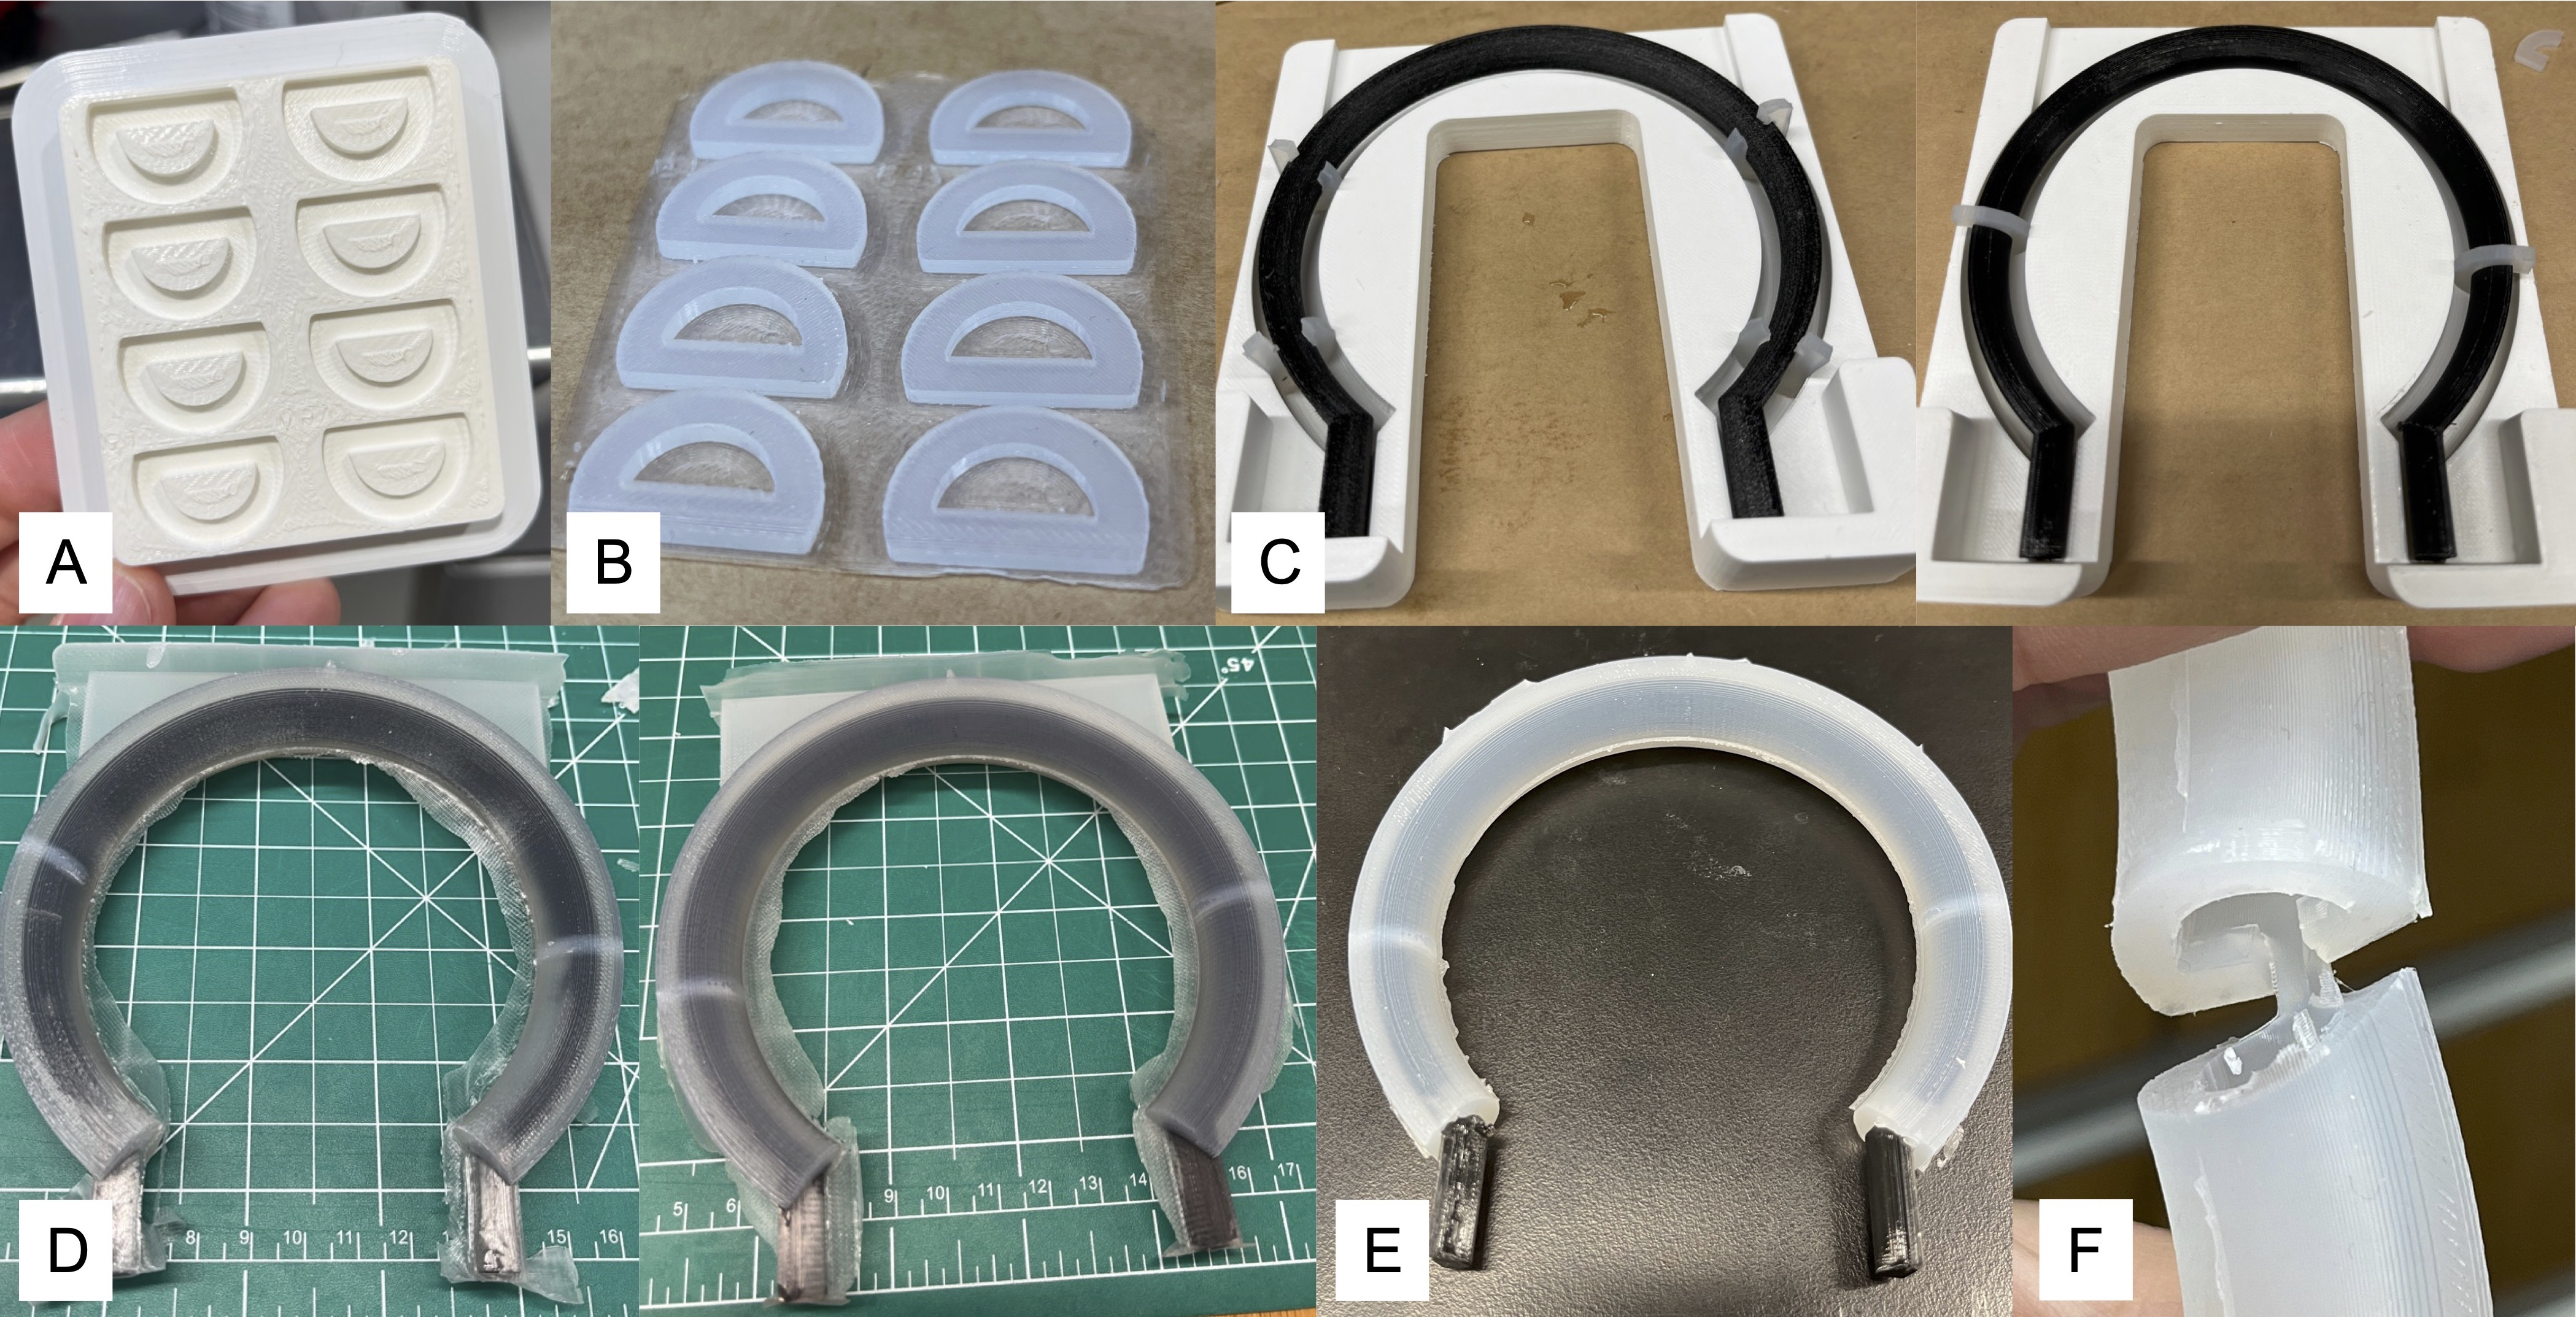
\includegraphics[width=6 in]{images4/ds20spacer.jpg}
    \caption{Images of failed attempts at using a spacer made from DS20 silicone to center the TPU insert. A. 3D printed mold for the spacers. B. casted spacers. C. Arbitrary placement of spacers. D. Casted actuators right after removing from the mold. E. After removing excess silicone. F. Failed attempt at creating a seal.}
    \label{fig:ds20spacer}
\end{figure}

\section{Mold Improvements}
The molds we 3D printed had served us well, but were beginning to buckle from the frequent clamping and tapping on the table to remove air from the actuators. The increase in flashing post each cast meant it was time to print new molds. The first upgrade was a larger pour hole with extra relief for the air bubbles that would get stuck at the top of the mold. Additionally, clamp placement needed to be on the parts where the two halves of the molds touch. If the clamp was tightened around an area meant to be filled with silicone, we noticed that the silicone walls would be uneven. Adding markings for safe places to apply the clamps improved wall thickness significantly. For the thinner silicones, extra clamps on the interior section were required to reduce leakage and flashing, as shown in Figure \ref{fig:newmolds}.

\begin{figure}[h]
    \centering
    \includegraphics[width=6 in]{images4/newmolds.jpg}
    \caption{Upgrades to the molds. A. Drawing of the larger pour hole. B. Drawing of the molds with markings for clamp placement. C. Photo of additional clamps required on the interior.}
    \label{fig:newmolds}
\end{figure}

\section{Case Study: Wax Inserts}
Creating an insert from wax was perhaps more trouble than it was worth, but it did lead us closer to the final fabrication method. We found three waxes compatible with curing silicone: Beeswax, paraffin wax, and microcrystalline wax. To cast the wax insert, we 3D printed a new mold and an insert out of PLA for casting a mold from silicone. We then casted the wax into the silicone mold. 

All three waxes were able to be partially casted and removed from the silicone mold. However, we found that the creating the wax insert to have the perfect cross section shape to ensure a future uniform cross section for the actuator to be difficult and the waxes were not rigid enough to hold their shape inside of the mold during casting. We thought about combining waxes in different ratios to enhance the stiffness and ease of casting, but even if the wax inserts were able to create the perfect cross section when casting silicone, they would have to be melted and recast for fabricating each actuator. With mass production in mind, we decided to not further pursue wax inserts. Figure \ref{fig:waxinserts} contains images from experimenting with wax inserts. 

\begin{figure}[h]
    \centering
    \includegraphics[width=6 in]{images4/waxinserts.jpg}
    \caption{Experimentation with wax inserts. A. 3D printed mold and insert for casting silicone mold for wax. B. Using popsicle sticks to hold insert above silicone while casting mold. C. Paraffin wax casted in silicone mold. D. Paraffin insert removed from mold. E. Beeswax and Microcrystalline wax cast in silicone molds. F. Beeswax and Microcrystalline wax removed from silicone molds}
    \label{fig:waxinserts}
\end{figure}

\section{Case Study: PCL Inserts}

PCL (Polycaprolactone) is a plastic that has a low melting temperature and is moldable with the use of warm water. Using the same silicone mold made for the wax inserts we used warm water to melt the PCL pellets into blobs which were pressed into the silicone mold. The DS20 mold was far too flexible to accurately shape the PCL. Also, as the pieces of PCL cooled and solidified, they would not fully bond with the other pieces, leaving air gaps in the insert. After tuning the timing between the pieces cooling down and adding more PCL pieces we were successful at creating an insert, and cast a DS20 actuator around the PCL insert. Unfortunately, the walls of the silicone were uneven and the PCL insert has the same single use problem as the wax inserts. Figure \ref{fig:pclinsert} contains photographs of experimenting with PCL as an insert and the DS20 actuator we casted using the PCL insert. 

\begin{figure}[h]
    \centering
    \includegraphics[width=6 in]{images4/pclinsert.jpg}
    \caption{Experimentation with PCL inserts. A. Silicone mold. B. An attempt. C. Melting PCL in warm water. D. PCL insert inside PLA mold. E. Casted around PCL insert. F. Removed from mold. G. Extra silicone removed. H. Final actuator.}
    \label{fig:pclinsert}
\end{figure}

\section{2 Part PLA Insert}
Feeling as though we were getting no where with creating an insert for the circular actuator, we revisited the good parts from the TPU insert: rigid enough to click into PLA molds, and flexible enough to be removed from the silicone after it cures. We had been operating under the assumption the insert should be one piece and the rectangular part that clicked into the mold must slide through the semi-circular cross section. We wanted an insert we could use repeatably that would create a constant cross section along the actuator. Inspired by the ability to remove the rectangular part from the PCL insert, we decided to split the PLA insert we printed for making silicone molds in half. We actually used a hacksaw. After filing the semi-circular faces of the now two-part PLA insert, we placed the pieces in and they felt fixed inside the mold, the only problem was the small gap which would create a bridge of silicone in the middle of the actuator. To resolve this, we quickly grabbed a piece of tape and cast an actuator around the 2 part PLA insert. We were concerned about removing the tape but proceeded forward. This actuator had even walls reminiscent of the PVA inserts. Post cure, with a small amount of IPA, both halves of the insert slid out and we were able to remove the tape with tweezers. While fabricating this actuator we were also iterating on attaching the fiberglass fabric and sealing it against the silicone, but that will be further detailed in future sections. Figure \ref{fig:twopartinsert} contains photos of the first actuator cast with a two part PLA insert. 

\begin{figure}[h]
    \centering
    \includegraphics[width=6 in]{images4/twopartinsert.jpg}
    \caption{First actuator made with a 2 part PLA insert. A. The insert held together with tape. B. Placed inside the mold. C. After silicone cast. D. After second silicone partially cast around fiberglass. E. Insert easily removed. F. Tape removed.}
    \label{fig:twopartinsert}
\end{figure}

So far, this was the most promising method for casting actuators with a reusable insert. To better connect and align the inserts, we added a connection point in the middle of the insert so that the two halves would fit together and also fit inside the mold. Because the casted silicone picks up the lines of filament, and 3D printing the inserts with the large overhang without support material would cause inconsistencies in the cross section, we attempted printing inserts in several orientations. After 3D printing, we would also file and sand the inserts to ensure a smooth surface for the silicone to cast around. To seal the interface between the two halves of the insert, we began using teflon tape which had a smaller width than the previously used yellow tape. After 3D printing inserts in several orientations, the final choice went to printing horizontally with support material, the same method used for printing the PVA and TPU inserts. Dozens of actuators were cast using this method. The final four silicones chosen for continuing characterization were DS20, DS30, SS40, and SS50. Figure \ref{fig:splitinsert} contains photographs of the possible orientations for 3D printing the split insert and actuators of the final silicones fabricated with this method. 

\begin{figure}[h!]
    \centering
    \includegraphics[width=6 in]{images4/splitinsert.jpg}
    \caption{Photographs of the 2 part insert method. A-C. Three orientations for 3D printing the insert. D-G. DS20, DS30, SS40, and SS50, respectively, cast using inserts printed in the orientation shown in C.}
    \label{fig:splitinsert}
\end{figure}

\section{Adding Strain Limiting Materials}
Now that we were able to consistently create circular actuators with a uniform cross section in a single pour, the next problem to solve was attaching the fiberglass fabric to the flat side of the silicone, a requirement for achieving the desired bending behavior with actuation. We used a large fiberglass fabric sheet and would cut it into strips to attach to the actuators. We used Sil-Poxy (Smooth-On) to adhere the fabric to the silicone. To ensure we added no stress to the silicone, we left the rigid PLA inserts inside the actuator while attaching the fiberglass fabric. The strips of fiberglass were cut slightly wider than the actuator to ensure that the entire flat face was covered in fibers. Additionally, the fibers were attached parallel to the actuator to ensure the strain would be limited axially. If the fiberglass was not attached properly, the actuator would bend and twist in different directions, which is preventable by properly attaching the fabric. 

Unfortunately, the Sil-Poxy adhesive was not strong enough to keep the fiberglass attached, so we had to develop a way of covering the fabric in silicone to ensure the fabric would not become loose against the exterior of the actuator. In the standard fiber-reinforced actuator, a thin wall of silicone is cast around the fiberglass, encasing the entire actuator. 

We attempted designing wider arch shaped molds so that we could cast another layer of silicone around the fiberglass, but this method was less than successful. It was difficult to ensure the second cast of silicone had no air bubbles and completely covered the actuator. Additionally, having to setup another large mold and make the walls of the actuator even thicker would require more air pressure to achieve the bending behavior. For the softer silicones, casting another layer would be possible, but for the thicker silicones such as SS40 and SS50, pouring another layer would be next to impossible. We considered casting an outer layer of a different material around the entire actuator, such as a thin Ecoflex silicone. Having the semi-circular cross section, the source of circumferential and radial strains that would impact the bending behavior, made from two different materials seemed unnecessary in the design of the circular actuator. 

Part of this project is not only designing an actuator that achieves a new bending behavior, but also simplifying the fabrication process for fiber reinforced actuators in general. With this in mind, we decided on using DragonSkin 10 (DS10) Fast cure silicone to paint a thin layer over the fiberglass fabric. The cure time for the DS10 silicone was under 1 hour and only a small amount is needed to encase the fiberglass without impacting the semi-circular cross section made from another silicone. This method was simple to execute repeatably and allowed for a consistent connection between the fiberglass fabric and the silicone actuator. Figure \ref{fig:fiberglass} contains photographs of actuators before adding the fiberglass and after coating the fabric with a thin layer of DS10 silicone. 

\begin{figure}[h!]
    \centering
    \includegraphics[width=6 in]{images4/fiberglass.jpg}
    \caption{Process of adding strain limiting fiberglass: A. Ensure the flat side of the actuator is flat. B. After adding fiberglass to an SS40 actuator. C. After adding fiberglass to a DS20 actuator. D. DS20 actuator right after the DS10 cured. E. After removing excess DS10.}
    \label{fig:fiberglass}
\end{figure}

\section{Sealing the Ends}
Once the fiberglass is attached and the DS10 is painted over, we seal both ends of the actuator. If using the Soft Robotics Toolkit method of attaching to the pressurization equipment, one end is sealed first, then the other end after attaching the hardware. 

The easiest method is using a cup full of silicone to seal each end of the actuator. While this method is the simplest, the amount of silicone pulled up the hollow actuator due to capillary effects is difficult to control. The larger the amount of silicone that forms the end cap, the more length that is lost from the final actuator. Decreasing the length of the actuator reduces the initial open angle of the circular actuator. Using a smaller sized cup with a small amount of silicone provides more control over the amount of silicone that forms the end cap. But the excess silicone cured around the end must be cut away, leaving an end that is not uniform with the rest of the actuator. 

To ensure only the necessary amount of material cures inside the end of the actuator to create the end cap, and to maintain the clean cross section of the actuator, we designed and 3D printed a mold that matches the curvature of the circular actuator. Using these molds allowed us to cap the ends of all of our actuators with the same thickness on each end, further ensuring uniformity between the actuators. Figure \ref{fig:endcaps} contains photographs of sealing the ends of the actuators and a drawing of the custom end cap mold used for the circular actuator. 

\begin{figure}[h!]
    \centering
    \includegraphics[width=6 in]{images4/endcaps.jpg}
    \caption{Methods for sealing the ends of the actuator. A. Using a cup full of silicone. B. Using a cup filled with less silicone. C. Using a smaller cup with even less silicone. D. A drawing of the custom mold used for the circular actuators. E. Sealing one end using the mold in D. F. Sealing both ends at once. }
    \label{fig:endcaps}
\end{figure}

\section{Connection to Pressurization Equipment}
To connect the actuator to the pressurization equipment, we used standard tubing with push-to-connect fittings that have 10-32 male threads. The Soft Robotics toolkit method for connecting fiber-reinforced actuators involves using 2 pieces of acrylic, a vented screw and a 10-32 nut to add tighten the acrylic pieces around the end cap of silicone. Installation requires puncturing the vented screw through the inside of the actuator. To connect the vented screw to the push-to-connect fitting, we use a 10-32 female standoff. 

This method was successful for softer silicones, such as DS20. However for stiffer silicones, puncturing with the vented screw often created a large hole in the end cap, which we attempted to seal with silicone glue, with varying success. Additionally, if we ever wanted to make the actuator longer and possibly spiral shaped, puncturing from the inside would prove difficult. 

To simplify the connection to the push-to-connect fitting, we designed and thanks to Sinisa Janjusevic, the machinist at Cooper, we were able to machine several barbs from brass stock with 10-32 female threads that directly connected to the push-to-connect fittings. There are multiple benefits to using the barb over the vented screw. Firstly, the barb provided a way to clamp the actuator during testing. Also, puncturing the actuator from the outside allowed us to further simplify the fabrication process because we could cast the silicone both end caps at the same time. Additionally, puncturing from the outside of the actuator provided more control over the location of the puncture hole because we could see the insertion point. 

To ensure an airtight connection, after puncturing the barb into the actuator, we used Sil-Poxy adhesive both underneath and around the brass barb. Also, we used a small amount of kevlar thread to tie the end cap around the spikes of the barb. Adding the thread proved to be the most effective way of ensuring an airtight connection. Figure \ref{fig:barb} contains photos of the vented screw method and our custom barbs for connecting the actuator to the pressurization equipment. 

\begin{figure}[h!]
    \centering
    \includegraphics[width=6 in]{images4/barb.jpg}
    \caption{Methods for connecting the actuator to pressurization equipment. A. Vented screw and inner piece of acrylic. B. Large puncture hole for the stiffer SS45 silicone. C. Airtight DS20 actuator. D. 10-32 female standoff and push-to-connect fitting. E. Barbs machined for the circular actuator. F. Direct connection to push-to-connect fitting. G. Airtight SS50 and DS30 actuators. }
    \label{fig:barb}
\end{figure}


\section{Fabrication Summarized}

To create the circular actuators we use a single-material casting procedure with 3D-printed molds. We chose a semi-circular cross-section for its small bending resistance \cite{polygerinos_modeling_2015}. To form the inner chamber, a two-piece insert snaps into the mold and comes apart for ease of removal (Fig.~\ref{figure:fab}A). The insert is constrained in the center of the mold so that the silicone walls have a constant thickness along the actuator to prevent off-axis motion (Fig.~\ref{figure:fab}B). To characterize how the actuator's behavior changes with material, we used four different silicones with Shore A Hardness ranging from 20--50: Dragon~Skin~20~(DS20), Dragon~Skin~30~(DS30), Smooth~Sil~940~(SS40), and Smooth~Sil~950~(SS50) (Smooth-On, USA). We mix, degas, and pour one of the two-part silicones inside the opening at the top of the mold (Fig.~\ref{figure:fab}C). After casting, we leave the silicone to cure at room temperature. 

After the silicone cures, we remove the actuator from the mold and cut away excess material (Fig.~\ref{figure:fab}D). We add a strip of fiberglass fabric (4 oz S-glass, US Composites) to the flat side of the cross-section with Sil-Poxy (Smooth-On, USA) (Fig.~\ref{figure:fab}E). The insert remains inside the silicone while attaching the fiberglass to ensure we add no additional stress. We paint a small amount of Dragon Skin 10 Fast (SmoothOn, USA) over the fiberglass to ensure a secure attachment to the actuator (Fig.~\ref{figure:fab}F). No other strain-limiting materials are required to achieve the bi-directional bending behavior, significantly simplifying the fabrication process. 

After removing the insert, we seal both ends with the same silicone used for the actuator body using a 3D-printed mold (Fig.~\ref{figure:fab}G). To create a secure connection to the pressure rig, we attach machined barbs by puncturing one side of the actuator. The interface is coated with Sil-Poxy to ensure an airtight connection (Fig.~\ref{figure:fab}H).

\begin{figure}[h!]
    \centering
     \includegraphics[width=5.5 in]{images4/fab.jpg}
    \caption{The simple fabrication process of the circular actuator.}
    \label{figure:fab}
\end{figure}
\chapter{Analytical Modeling}

\section{Overview}
First, we must define \emph{bending} to model the actuators' bending behavior with varying input pressure. We define the bending angle of the actuator at any pressure based on the \emph{open} angle formed by the strain-limiting layer, the fiberglass fabric. For each bending angle, we calculate the strain throughout the actuator to maintain the angle formed by the fiberglass layer. We calculate the stress within the actuator based on the material model for the hyperelastic silicone. Once we know the stress in the material, we can calculate the pressure required to induce the stress. 

In preliminary models, we focused on shapes the fiberglass fabric could form, assuming it maintains a constant curvature. The final model included the circumferential and radial strains within the actuator to calculate the pressure required for a bending angle assuming constant curvature along the length of the actuator. 

\section{Preliminary Model \& Visualization}

Starting with the length of the fiberglass fabric, the circular shape of the actuator, and the largest open angle we could fabricate, we developed a simple method of plotting the shape of the actuator and determining the maximum axial strain. While first attempting to model the circular actuator's bending behavior, we had yet to realize that the actuator was capable of bi-directional bending. Nor did we know that the actuator was unstable at the infinite curvature position. All we knew then was the length of the fiberglass fabric and that the actuator was a circle. 

\begin{figure}[ht]
    \centering
    \includegraphics[width=3 in]{images5/lnot.jpg}
    \caption{Drawing containing the initial bending angle, and length of the fiberglass fabric highlighting the length lost to the fabrication process.}
    \label{fig:lnot}
\end{figure}

During fabrication, we lose a non-significant amount of the actuator's length to seal the ends. Fig. \ref{fig:lnot} contains the variables and shows the length of the actuator lost to fabrication. The initial bending angle, $\psi_{0}$, ranged between 215-230$^\circ$. The circle formed by the fiberglass layer has a radius, $r_{0}$, of 2.4~in or 6.1~cm. We can calculate the length of the fiberglass fabric, $l_{0}$, using $l_{0} = r_{0}*\psi_{0}$, the arc length equation for a circle. 

For a given $l_{0}$, we can visualize how reducing $\psi$ increases the bending radius, $r$. As $\psi$ approaches $0^\circ$, the bending radius approaches infinity. Fig. \ref{fig:unbending} displays the first visualization of the actuator's bending behavior as $\psi$ approaches $0^\circ$. This model assumes that the actuator maintains a circular shape. 

\begin{figure}[ht]
    \centering
    \includegraphics[width=3.5 in]{images5/unbending.jpg}
    \caption{First visualization of the unbending behavior of the circular actuator assuming constant curvature of the fiberglass fabric.}
    \label{fig:unbending}
\end{figure}

Assuming the actuator undergoes no circumferential or radial strain is a bold assumption, considering we add no strain-limiting materials around the cross section during fabrication. However, it is helpful to consider each line of silicone undergoing axial strain. If we assume the semi-circular cross-section does not change during pressurization, we can visualize the strain of the innermost line of silicone. We plotted a few samples: the black lines represent the fiberglass layer, and the colored lines represent the strained, innermost silicone layer. Fig. \ref{fig:innermoststrain} contains samples to visualize each line of silicone and the axial strain it must undergo to maintain the constant cross-section, length, and bending angle set by the fiberglass layer. 

\begin{figure}[ht]
    \centering
    \includegraphics[width=3.5 in]{images5/innermoststrain.jpg}
    \caption{First visualization of the axial strain the innermost line of silicone must undergo to maintain the cross section and curvature set by the fiberglass layer.}
    \label{fig:innermoststrain}
\end{figure}

\section{A Discovery}

While inflating the actuators during initial testing, we discovered that adding more air pressure past the limit where $\psi$ approaches 0$^\circ$ caused the actuator to continue bending. The silicone of the semi-circular section continued expanding, and the additional axial strain added curvature back to the fiberglass fabric. In an accident where we added too much pressure to the actuator, we discovered the circular actuator's bi-directional bending capabilities. We accidentally created a fiber-reinforced actuator capable of two bending directions with a single positive pressure source. After making this discovery, we had to alter the definition of a bending angle to build a continuous model over the entire range of motion. Introducing negative bending angles to define the curling behavior did the trick. The following section will fully define the analytical model for the circular actuators' entire range of bending behavior. 

\section{Analytical Model for Bending Angle}

To characterize the actuator's bending behavior as a function of input pressure and material properties, we developed an analytical model for curling and uncurling based on those found in \cite{polygerinos_modeling_2015, connolly_automatic_2017, hu_precurved_2022}. We calculate the input pressure $P$ required to reach a given bending angle $\psi$ using the geometry of the actuator, the length of the inextensible layer $l_0$, and the non-linear hyperelastic material properties of each silicone, including non-axial deformation. To account for circumferential deformation, we transform the cross-section at each pressure based on material stretches. As the pressure increases, the actuator uncurls (decreasing $\psi$) from its initial bending angle $\psi_0$ to an angle $\psi=0$, where the actuator is straight. Further increasing pressure causes $\psi$ to become negative, corresponding to curling behavior, thus generating a bi-directional range of motion. Fig. \ref{fig:modelall} contains all of the variables used in the analytical model. 

\begin{figure}[ht]
    \centering
     \includegraphics[width=6 in]{images5/modelall.jpg}
    \caption{Geometric variables defined for the analytical model. The thicker line represents the inextensible layer. A. Definition of positive and negative bending angles. B. Undeformed cross-sectional geometry of the actuator. C. Axial stretch ratios and corresponding stress in response to applied pressure. D. Deformed cross-sectional geometry to account for circumferential and radial deformation.}
    \label{fig:modelall}
\end{figure}

\clearpage
\subsection{Stretch Ratios}

As the actuator bends, the silicone stretches in the axial direction to maintain the length $l_0$ of the inextensible layer. The model assumes that the actuator maintains a single, constant bending radius along its length at all pressures and that the cross-section remains orthogonal to the inextensible layer. We also assume incompressibility in the hyperelastic material, such that $\lambda_{1}\lambda_{2}\lambda_{3} = 1$ where $\lambda_i$ is the stretch ratio in each direction (axial, circumferential, and radial, respectively). This assumption requires that the cross-sectional area of the silicone remains constant, even as the shape deforms. Increasing pressure causes the semi-circular region to expand outwards into a circular shape, resulting in thinning of the actuator's walls to maintain a constant cross-sectional area (Fig. \ref{fig:modelall}D). We assume no geometric changes in the base layer because of the proximity to the inextensible layer.

For the undeformed cross section, as shown in Fig.~\ref{fig:modelall}B, $\beta$ is the coordinate in the base layer away from the inextensible layer, and $\tau$ is the distance from the inner wall in the $\varphi$ direction. The base region has thickness $b$~=~0.38~cm, and the undeformed semi-circular cross-section wall has radius $a_0$~=~0.64~cm and thickness $t_0$~=~0.38~cm. In the deformed cross-section (Fig.~\ref{fig:modelall}D), we assume that the silicone forms a circular arc with offset from the base $q$, inner radius $a$, wall thickness $t$ and angle range $-\varphi_m$ to $\varphi_m$. $\tau'$ and $\varphi'$ are scaled coordinates with reference to the undeformed shape such that $\tau'=\tau\frac{t}{t_0}$ and $\varphi'=\varphi\frac{2\varphi_m}{\pi}$.

For a given bending angle $\psi$, we calculate the axial stretch ratio $\lambda_1$ as $\lambda_{\beta}$ for material in the base and $\lambda_{\varphi,\tau}$ in the semi-circular region (Fig.~\ref{fig:modelall}C). When $\psi$ is negative, the axial stretch ratio remains positive as all lengths must exceed $l_0$. We also calculate the circumferential stretch ratio based on the deformed cross-section. These equations hold for the entire range of $\psi$ and deformation of the cross-section. 

\begin{equation}
    \lambda_1=\lambda_{\beta} = \frac{l_{0} - \beta \psi}{l_{0}-\beta\psi_0} 
    \label{eq:stretchbeta}
\end{equation}

\begin{equation}
    \lambda_1=\lambda_{\varphi,\tau} = \frac{l_{0} - (b+q+(a+\tau')\cos\varphi')\psi}{l_{0} - (b+(a_0+\tau)\cos\varphi)\psi_{0}}
    \label{eq:stretchphitau}
\end{equation}

\begin{equation}
    \lambda_2=\lambda_c = \frac{2(a+\tau')\varphi_m}{(a_0+\tau)\pi} 
    \label{eq:stretchc}
\end{equation}

For the undeformed shape, the circumferential stretch ratio $\lambda_2$ is 1. The stretch ratio in the radial direction $\lambda_3=\lambda_r$ can be calculated as $\lambda_3=1/(\lambda_1 \lambda_2)$ from the incompressibility assumption. To find the wall thickness $t$ of the circular arc region of the deformed cross-section, we integrate the radial stretch of the undeformed shape over the thickness:

\begin{equation}
    t = \int_0^{t_0} \frac{1}{\lambda_{\varphi,\tau} \times 1} d\tau 
    \label{eq:thicknessfromlambdar}
\end{equation}

To account for the inaccuracy of the material models and the compressibility of the DragonSkin materials, we scale the calculated thickness by $k_t(1-|\psi-\psi_0|/\psi_0)$ where $k_t = 0.3$ is a constant determined by best fit to the experimental expansion results. This scaling accounts for the non-zero radial stress, especially at negative bending angles. No scaling is necessary for the stiffer SmoothSil materials. 

To transform the cross-section from the original semi-circle to the circular arc, we use the scaled thickness $t$ and the cross-sectional area $A_0$ to calculate the deformed inner radius $a$, angle range $2\varphi_m$, and vertical offset $q$:

\begin{equation}
    \frac{A_0}{2\sin{\varphi_m}t}-\frac{t}{2}=\frac{a_0}{\sin{\varphi_m}}
    \label{eq:phi_m}
\end{equation}

\begin{equation}
    a=\frac{A_0}{2t\varphi_m}-\frac{t}{2}
    \label{eq:a_aug}
\end{equation}

\begin{equation}
    q=-a\cos{\varphi_m}
    \label{eq:q_aug}
\end{equation}

The axial and circumferential stretch ratios are then recalculated using the deformed cross section and Equations \ref{eq:stretchbeta}--\ref{eq:stretchc} before calculating stress with the material models.

\subsection{Converting Strain to Stress}

To describe the stress-strain relationship for each of the soft materials, multiple material models are available; they can vary significantly in accuracy depending on the amount of strain \cite{paterno_hybrid_2018}. We choose the Ogden hyperelastic material model because it is more accurate at higher stretches and for softer materials \cite{marechal_toward_2021}. The strain energy density function $W$ for the Ogden model is given by Eq. \ref{eq:strain-ogden}, where $\mu_{p}$ and $\alpha_{p}$ are experimentally determined material coefficients. We can use a given Neo-Hookean material model coefficient ($\mu$) in the Ogden model by setting $N=1$ and $\alpha_1=2$. 

\begin{equation}
    W=\sum_{p=1}^N \frac{\mu_p}{\alpha_p}(\lambda_1^{\alpha_p}+\lambda_2^{\alpha_p}+\lambda_3^{\alpha_p}-3)
    \label{eq:strain-ogden}
\end{equation}
\\
The Cauchy stresses in all three directions are given by $\sigma_j=-p+\lambda_j\frac{\partial W}{\partial\lambda_j}$, where $p$ is a Lagrange multiplier. The stresses in the radial direction are significantly smaller than those in the other directions, so we assume $\sigma_3=0$. We calculate the axial and circumferential stresses using Equations \ref{eq:s_1} - \ref{eq:multiplier-p} and the material properties found in Table \ref{table}. 

\begin{equation}
    \sigma_1 =-p+\mu_1\lambda_1^{\alpha_1}+\mu_2\lambda_1^{\alpha_2}+\mu_3\lambda_1^{\alpha_3}
    \label{eq:s_1}
\end{equation}

\begin{equation}
    \sigma_2 =-p+\mu_1\lambda_2^{\alpha_1}+\mu_2\lambda_2^{\alpha_2}+\mu_3\lambda_2^{\alpha_3}
    \label{eq:s_2}
\end{equation}

\begin{equation}
    p=\mu_1(\lambda_1\lambda_2)^{-\alpha_1}+\mu_2(\lambda_1\lambda_2)^{-\alpha_2}+\mu_3(\lambda_1\lambda_2)^{-\alpha_3}
    \label{eq:multiplier-p}
\end{equation}

\begin{table}[h!]
\caption{Material Properties Used in Analytical Model}
\label{table}
\centering
\begin{tabular}{l r r l}
\hline
{} & \bfseries Variable & \bfseries Value & \bfseries Unit \\
\hline\hline
DS20 \cite{marechal_toward_2021} & $\mu_1$, $\mu_2$, $\mu_3$ & -0.9534, -1.4515, 2.4085 & MPa\\
{} & $\alpha_1$, $\alpha_2$, $\alpha_3$ & 3.478, 3.181, 3.339 & {}\\
\hline
DS30 \cite{marechal_toward_2021} & $\mu_1$, $\mu_2$, $\mu_3$ & 0.03816, 0.02524, 0.04456 & MPa\\
{} & $\alpha_p$ & 3.417 & {}\\
\hline
SS40 \cite{pagoli_review_2022} & $\mu_1$ & 0.24 & MPa\\
{} & $\alpha_1$ & 2 & {}\\
\hline
SS50 \cite{xavier_finite_2021} & $\mu_1$ & 0.68 & MPa\\
{} & $\alpha_1$ & 2 & {}\\
\end{tabular}
\label{table}
\end{table}

\clearpage
\subsection{Pressure from Bending Moments}

The bending moments $M_P$ and $M_\sigma$ about the \(O\) axis (Fig.~\ref{fig:modelall}C) result from pressure on the end of the actuator and axial stress, respectively. These moments must be equivalent for the actuator to achieve static equilibrium. We calculate the bending moment $M_\sigma$ as the integral of the force from axial stress in both the base ($\sigma_{\beta}$) and the circular arc ($\sigma_{\varphi, \tau}$) regions times the orthogonal distance from \(O\) for the entire length of the actuator. 

\begin{equation}
    M_{\sigma} = 2l_{0} \int_{0}^{b} \sigma_{\beta} (a_0+t_0) \beta  d\beta
    + l_{0}\int_{0}^{t_0}\hspace{-2px}\int_{-\frac{\pi}{2}}^{\frac{\pi}{2}}\hspace{-2px}\sigma_{\varphi,\tau}((a+\tau')\cos{\varphi'}+b+q)(a+\tau') d\varphi d\tau
    \label{eq:moment-axial}
\end{equation}

The bending moment $M_P$ resulting from a given input pressure \(P\) acting on the end of the actuator is a function of the deformed cross-sectional geometry: 

\begin{align}
    M_P & = P \int_{-\frac{\pi}{2}}^{\frac{\pi}{2}}\int_0^{a} a(b+q+a\cos{\varphi})d\varphi da \\ \nonumber \\
    & = \frac{4 a^{3} + 3 \pi a^{2} (b+q)}{6} P 
    \label{eq:moment-p}
\end{align}

We equate (\ref{eq:moment-axial}) and (\ref{eq:moment-p}) and solve for the required input pressure $P$ to induce the axial stresses for a given bending angle $\psi$. To account for the underestimation of $P$ due to uncertainty in the material models and non-uniformity in the actuator, we scale the calculated pressure by a constant $k_P$, determined by a best fit for each material. $k_P$ is 3.8 for DS20, 1.8 for DS30, and 2.2 for SS40 and SS50. 
\chapter{Pressure Rig}

\section*{Preface}

Thank you to Michael Giglia and Isaiah Rivera, the design and construction of the pressure rig would not have been possible without their contributions. 

\section{Overview}

We designed the pressure rig to actuate and control the pressure inside the soft robots presented in this work. The rig contains an air tank reservoir that stores pressurized air generated from a compressor. The reservoir supplies air to a pressure regulator that controls the input pressure of the soft robot. A microcontroller ($\mu$C) controls both the regulator and compressor. The computer running the test script either takes a photograph or a force reading at each pressure increment. Fig \ref{fig:blockdiagram} contains a block diagram detailing the pressure rig and the sensors used to characterize the behavior of the circular actuators. This chapter details the mechanical components, the electrical components, firmware on the microcontroller through two iterations of the rig, and the testing scripts used to characterize bending angle and blocked force. 

\begin{figure}[ht]
    \centering
    \includegraphics[width=5.5 in]{images6/blockdiagram.jpg}
    \caption{Block diagram of the pressure rig showing the path of compressed air, the relevant control signals, and the sensors used for characterization of the circular actuator.}
    \label{fig:blockdiagram}
\end{figure}

\section{Air Supply Components}

The air tank reservoir (LYH-1004, Longyihong) has a half-gallon capacity rated for 200 PSI, well over any pressures used in this work. On each side of the tank, there is a 1/4" NPT port. One side of the tank is connected to the compressor (202, GSPSCN). On the other side of the tank, we use a 2-way, 5-port manifold block (ML-G, Baomain) to connect one of the pressure sensors, the supply of the pressure regulator, the 45 PSI pressure-relief valve (9889K19, McMaster) and the 0-50 PSI gauge (0-50PSI HF, Meanlin Measure). 

The pressure regulator (ITV1031-21N2N4, SMC) requires a 12V power supply and an input signal of 0-5V for the pressure on the output. The display shows the pressure in PSI. Both the pressure regulator and the compressor are powered by a rechargeable 12V lead-acid battery (ML5-12, Mighty Max Battery). We charged the battery often to maintain its health. We placed an E-Stop button (YW1B-V4E02R-BOX, Twtade) between the battery and the regulator. Fig. \ref{fig:airsupply} contains a photograph of the pressure rig with labeled air supply components. 

To ensure no air leaks occurred, we used Teflon Tape to secure the connections between the components. We used white 1/4" diameter tubing and 1/4" NPT to 1/4" OD tubing push-to-connect fittings (PC-1/4-N2, Tailonz Pneumatic) to connect the manifold block to the pressure regulator and pressure sensor. We used laser-cut acrylic pieces and standoffs to lift all of the components off the metal testing table. 

\begin{figure}[ht]
    \centering
    \includegraphics[width=3.5 in]{images6/airsupply.jpg}
    \caption{Photograph of the pressure rig with air supply components labeled.}
    \label{fig:airsupply}
\end{figure}

\section{Pressure Sensor}

The differential pressure sensor (MPX2200DP, Freescale Semiconductor) measures the pressure within the air tank to ensure the regulator has sufficient air supply. We used readings from this sensor to turn the compressor on or off. To connect the pressure sensor to the microcontroller, we used an instrumental amplifier (INA125P, Texas Instruments) and a 13-bit analog-to-digital converter with an SPI serial interface (MCP3301, Microchip). Both microcontrollers had SPI communication libraries written to interface with the pressure sensor. 

\section{Compressor Control}

We designed the compressor to be controlled by the microcontroller using a digital pin connected to an NMOS (IRF540N), which connects to a relay to connect the compressor to the battery. Using the pressure sensor reading of the air tank, we wrote a state machine that controls the pressure so that the tank remains full while testing the actuators. Fig \ref{fig:compressorsm} contains a diagram of the state machine that runs on either microcontroller to control the compressor. 

\begin{figure}[ht]
    \centering
    \includegraphics[width=6 in]{images6/compressorsm.jpg}
    \caption{State machine diagram for compressor control to fill the air tank.}
    \label{fig:compressorsm}
\end{figure}

The state machine has 3 states, compressor OFF (state 0), compressor ON (state 1), and ESTOP (state 2). While in state 0, we check if the current pressure reading in the tank is less than the desired pressure minus some tolerance. If the pressure has dropped below this amount, switch to state 1, and the compressor turns on. In state 1, we check if the dP/dt (the change in pressure over time) is satisfactory, such that we know there is no air leak. We use timing functions in firmware to check the current pressure compared to the pressure reading each time increment before. If dP/dt is less than expected, we can assume there is a leak and the compressor is not filling up the tank; in this case, switch to state 2, the emergency stop state. If dP/dt increases as expected, check if the current pressure is above the desired pressure plus some tolerance. If so, switch to state 0 and turn the compressor off. 

The allowable tolerance of the tank pressure provides a small buffer, ensuring the compressor does not turn on and off frequently, prolonging its life. We used 36~$\pm$~4~psi (250~$\pm$~35~kPa) as the desired tank pressure for experimentation. 

\section{Input to Pressure Regulator}

The regulator's output pressure range is programmable. To stay within the release valve's bounds, we set the output pressure to be between 0 and 40 PSI. 
The analog input signal (0-5V) has a linear relationship between voltage and output pressure from the regulator. We used a digital potentiometer with an SPI serial interface (MCP4251-103E/P, Microchip) connected to the Arduino (ELEGOO UNO R3) in the first iteration. In the second iteration, we used a 12-bit digital-to-analog converter, also with an SPI interface, connected to the Pico microcontroller (Raspberry Pi). 

\subsection{Sending Pressure Commands to Arduino}

Using an Arduino microcontroller, we controlled the digital potentiometer, creating the analog voltage signal that controls the pressure output from the pressure regulator. The microcontroller and the digital potentiometer communicated over SPI. However, we wanted to be able to set the desired pressure using the computer running the test script. The computer connects to the camera and force sensors. We wrote the testing script in Python to step between pressure increments so that we could either take a photograph of the bending angle or record the blocked force using the load cell. In between taking a photograph or force reading, the computer sends pressure commands to the microcontroller to change the pressure inside the actuator. 

We used a custom g-code-like serial protocol Michael Giglia had previously implemented and modified it to send the desired pressure commands. At the time, we were using the 8-bit signal to the digital potentiometer, so the message sent from the Python script to the $\mu$C was a number between 0-255. After determining the appropriate commands and the pressure output at those commands, we wrote a testing script that would iterate through each pressure command and take a photograph or force reading when the person taking the data indicated that the actuator had reached a steady state at that pressure. 

\subsection{Problems with the Digital Potentiometer}

The digital potentiometer used to create the analog voltage as the input signal to the pressure regulator was problematic due to the non-linear results of controlling it with the Arduino. 

To set the pressure in the actuator, we sent an 8-bit command (0-255) from the computer running the test script to the Arduino. We attempted to characterize the non-linear relationship between the range set on the pressure regulator, the command sent to the digital potentiometer, and the output pressure. Fig. \ref{fig:bitpressuremap} contains the pressure readings based on the command sent to the digital potentiometer at 4 different ranges of the pressure regulator. Because the resolution at higher pressures was significantly lower, we increased the range on the pressure regulator to gain more resolution at higher pressures. The silicone actuators were highly sensitive to pressure changes, and we found worse hysteresis in the bending angle when the pressure increments were highly uneven. 

\begin{figure}[ht]
    \centering
    \includegraphics[width=5 in]{images6/bitpressuremap.jpg}
    \caption{Relationship between the range set on the pressure regulator, the command sent to the digital potentiometer and the output pressure in the actuator for four pressure ranges.}
    \label{fig:bitpressuremap}
\end{figure}

\subsection{Digital to Analog Converter}

It was critical to have linear control over the output pressure of the pressure regulator to increase or decrease the pressure in the actuator by an even amount. To achieve linear output pressure, we needed a way to create an analog 0-5V signal with linear input commands with the desired output pressure. We achieved linear control between the command and the output pressure by implementing a 13-bit digital-to-analog converter (MCP4921-E/P, Microchip) using an SPI interface with a Pico microcontroller. This upgrade allowed us to measure the circular actuator's bending and blocked force behavior with even pressure increments, critical to minimizing hysteresis during characterization. 

\subsection{Problems with Switching to the Pico}

Switching microcontrollers required a complete overhaul of the testing software and firmware. Isaiah Rivera rewrote and rebuilt the pressure rig to have the upgraded microcontroller driving it. Still, because we switched to the digital-to-analog converter to control the regulator's output, we had to write the SPI communications for the new device, and we wanted to move to the Pico. Hence, we decided to upgrade the entire rig. 

Due to time constraints and an oversight of how much development would be required to change microcontrollers, we simplified the pressure rig. We used one Pico $\mu$C to control the compressor. The pressure sensor interface and compressor control state machine always ran while the rig was on. We used a second Pico $\mu$C to interface with the pressure regulator. Instead of waiting for the serial protocol implementation, we decided to use a potentiometer input, using the Pico's analog-to-digital converter to control the pressure output of the regulator. While this solution certainly requires several layers (a 3.3V analog signal is read by the Pico, converted to a digital value, and sent over SPI to a digital-to-analog converter, which creates a 0-5V analog signal to set the regulator's pressure), it did work. It allowed us to take both bending angle data and blocked force data at even pressure increments, which was the most important part of characterization. 

We discretized the potentiometer readings into even increments to ensure the same pressure commands were sent for each actuator's test. The new setup using the digital-to-analog converter provided immense resolution on the pressure regulator's output, but we wanted to use 1 psi increments. Since now the relationship between the signal sent to the DAC and the pressure output on the regulator was linear, it was simple to discretize the values so that we had even increments of 1.0$\pm$0.1 psi. 

Since we had lost the serial protocol between the $\mu$C and the computer, the testing script had to be modified to print the desired pressure to the terminal output. The person running the test would turn the potentiometer until the regulator received the desired pressure command. A photo or force reading could be taken once the actuator had reached a steady state. Despite taking slightly longer to run each test, the hysteresis caused by uneven pressure increments was greatly reduced, making the switch to the Pico worth it. 

\section{Camera for Bending Angle}

To experimentally measure the bending angle of the circular actuators, we used a camera to take photos of the actuator at each pressure. We entertained using a flexible resistor (SEN-08606, SparkFun), but this would not provide insight into variations in curvature or non-axial expansion along the length of the actuator. A photograph, although requiring post-processing, provides infinite insight into the actuator's bending behavior. 

We used a web camera (C920 Hd Pro, Logitech) to take photographs of the actuator at each pressure. Our testing script used OpenCV \cite{opencv_library} to interface with the web camera and save the photographs in the appropriately named directory for later post-processing. 

For each test, the person running the test would input the \emph{name} of the actuator and the number of the test. For example, DS20K3\textunderscore4 meant the actuator was made of DragonSkin 20 silicone, it was fabricated with the K method (the insert split in the center of the actuator), it was the third actuator made with this material and fabrication method, and this is the fourth time running the bending angle experiment. 

Using the terminal output and keyboard of the computer, the person running the test would see the pressure about to be sent to the actuator and then press the space bar to confirm the pressure should be changed. Once the actuator had reached a steady state at that pressure, pressing the "m" key would take a photograph, name it with the name of the actuator and the current pressure, and save it to a directory with the name of the test. The script would continue through the list of pressures we wanted to test the actuator at until the peak pressure was reached. After documenting the bending angle at the maximum pressure, the pressure would reverse to capture hysteresis in the bending behavior. Each test took 5-10 minutes to take 30-35 photographs, depending on the achievable peak pressure in the actuator. Chapter \ref{chapter:bendingangle} fully details capturing the bending angle of the the circular actuator. 

\section{Load Cell for Blocked Force}


\chapter{Measuring Bending Angle}

\section{Iterations on Orientation}

As with everything related to this project of designing and characterizing a new type of soft robotic actuator, discovering how to measure the bending angle at different pressures repeatably took several iterations. Even with just the preliminary models, we knew that the actuator would unbend with increasing pressure. We needed to develop a way to hold the actuator in front of the camera so we could measure the bending angle and compare it to the model. 

We measured the curvature and calculated the bending angle from the fiberglass fabric embedded into the actuator, so we knew that the fabric must be perpendicular to the camera's view. We also wanted to capture the actuator's circumferential expansion in the photographs. Before we developed the brass barbs, which provided a part of the actuator we could easily clamp to, we needed to figure out how to fix the actuator in front of the camera to capture the bending behavior. 

\subsection{First Testing Orientation}

For the first test, the materials available were a scrap piece of matte black acrylic, a triangle we fastened to the lab table, and an aluminum extrusion to hold the acrylic upright against the triangle. We placed the 10-32 female standoff used to inflate the actuator inside a hole on one side of the triangle, and we ran the air supply tube through the triangle to hold the actuator in place. We placed the camera far enough away from the actuator so that the pressure reading (in psi) on the regulator was visible in the photo because we were still working on the communications between the regulator and the microcontroller. The first actuator photographed was DS20 silicone fabricated with a two-part insert split in the center of the actuator. We used $1.0~\pm~0.1$ increments from 2.0 to 12.0 psi to capture the bending behavior. The photographs taken are in Fig. \ref{fig:firstdataset}. 

We identified several problems with capturing the bending angle using this orientation. Based on the model, we expected the actuator to have constant curvature at each pressure, and having the fiberglass side rest on the flat table introduced reductions in curvature; the portion of the silicone touching the table was flatter than the rest of the actuator. Additionally, the end of the actuator was pulled down by gravity, increasing the curvature and inducing a larger bending angle, $\varphi$. 

\begin{figure}[h]
    \centering
     \includegraphics[width=6 in]{images7/firstdataset.jpg}
    \caption{First photos taken to observe the bending angle of the circular actuator. Pressure increments are $1.0~\pm~0.1$ from 2.0 to 12.0 psi.}
    \label{fig:firstdataset}
\end{figure}

\clearpage

The effects of gravity in this testing orientation were worse on the stiffer silicones. Fig. \ref{fig:ss45fallsover} contains 3 sample images at 2.0, 9.2, and 12.8 psi of an SS45 actuator photographed in the first testing configuration. Note that the actuator fell over while taking the middle photograph. Even though we did not fully model the SS45 silicone actuators, primarily due to lack of material properties for this material, we were able to capture the difference between 12 psi for a DS20 actuator compared to one with over double the shore hardness. 

\begin{figure}[h]
    \centering
     \includegraphics[width=6 in]{images7/ss45fallsover.jpg}
    \caption{Photos of a SS45 actuator at 2.0, 9.2, and 12.8 psi.}
    \label{fig:ss45fallsover}
\end{figure}

Despite these photographs being unusable for capturing the bending behavior, we did learn a few things from how the circular actuator behaves. The discoloration near the center of the actuator is from the Teflon tape used to seal the gap between the two halves of the insert. We did not know then that the silicone was not curing all the way in the areas where the tape touched the silicone. Additionally, the minor change in wall thickness in this region of silicone would cause significant variations in circumferential and radial expansion in the center of the actuator. This variation led to more circumferential expansion, causing more axial strain, which caused an increase in curvature in the center of the actuator, further reducing the constant curvature expected from the model. Moving the split of the insert to the edge of the actuator, an area of silicone that we would cut away before sealing the ends, significantly improved the bending behavior. 

\subsection{First Horizontal Testing}

In an attempt to remove the effects of gravity on the curvature of the actuator, we placed the camera pointing down at the table. This testing orientation did remove the inconsistencies created by having the actuator rest flat on the table and gravity pulling the end. However, friction now significantly impacts bending behavior. The bending angle varied significantly compared to vertical testing. Fig. \ref{fig:ds20h} contains images of a DS20 actuator with increasing psi. 

\begin{figure}[h]
    \centering
     \includegraphics[width=6 in]{images7/ds20h.jpg}
    \caption{Photos taken of a DS20 actuator at various psi pressures when placed horizontally on the lab bench.}
    \label{fig:ds20h}
\end{figure}

\subsection{Unbending with Gravity}

In an attempt to remove friction from restricting the decrease in bending angle with increasing pressure, we entertained adding the effects of gravity to the model as an additional bending moment affecting the curvature of the actuator. After testing in this configuration, we quickly determined that gravity-induced non-trivial variations in the curvature along the length of the actuator. Especially at lower pressures, the actuator lost its circular shape due to the effects of gravity. At higher pressures, the actuator was able to hold the straight position. During these tests, we were still not going above 14.6 psi when $\varphi=0$ because we had yet to discover the negative bending angle capabilities of the circular actuator. Fig \ref{fig:withgravity} contains photographs of a DS20 actuator held at the top so it could unbend with the help of gravity. This test removed friction's effects because nothing touched the actuator except the clamp on the brass barb. 

Comparing DS20 and DS30 at the same pressure values, DS20 has a lower bending angle, which we expected because the silicone requires more stress to achieve the same strain. Fig \ref{fig:d30withgravity} contains photographs of a DS30 actuator at the same pressure increments. This DS30 actuator displayed some twisting motion as the pressure increased. The twisting is likely due to the fibers of the fiberglass fabric not being aligned with the actuator, or the insert could have been slightly misaligned in the mold, causing uneven wall thickness, which would cause uneven strains, inducing the twisting behavior.

\begin{figure}[h]
    \centering
     \includegraphics[width=6 in]{images7/withgravity.jpg}
    \caption{Photos taken of a DS20 actuator at various psi pressures when held vertically.}
    \label{fig:withgravity}
\end{figure}

\begin{figure}[h]
    \centering
     \includegraphics[width=6 in]{images7/d30withgravity.jpg}
    \caption{Photos taken of a DS30 actuator at various psi pressures when held vertically.}
    \label{fig:ds30withgravity}
\end{figure}

\clearpage
\subsection{Vertical but Above Table}

After testing with gravity assisting the bending behavior, we attempted once again to photograph the bending angle vertically. This time, we raised the actuator using standoffs to reduce the restrictions on curvature from previous experiments in this orientation. Additionally, the test script was modified to both increase and decrease the pressure inside the actuator so that we could capture the hysteresis of the bending angle. Unfortunately, now that the table was not there to support the actuator, gravity not only pulled the actuator so that it touched the table at low $\varphi$ but added an incredible hysteresis to the bending behavior. Fig \ref{fig:ds20sver} contains photographs of a DS20 actuator against a blue and black checkerboard background. The images on the left are increasing the pressure, and those on the right are decreasing the pressure. While decreasing the pressure, the actuator maintained significantly lower $\varphi$ than previously observed when increasing the pressure. 

\begin{figure}[h]
    \centering
     \includegraphics[width=6.5 in]{images7/ds20sver.jpg}
    \caption{Photos taken of a DS20 actuator vertically but offset from the table with standoffs. The left group was increasing the pressure, and the right group was from decreasing the pressure.}
    \label{fig:ds20sver}
\end{figure}

\clearpage
\subsection{Unbending Against Gravity}

In yet another attempt at finding an orientation where we could measure the bending angle of the circular actuator without the effects of friction or restrictions from the table, we tested actuators unbending against gravity. We accidentally put 25 psi into a DS20 actuator during testing. We feared that the actuator would explode, but it did not! The actuator continued bending past $\varphi=0^\circ$ and continued what we defined as the negative $\varphi$ bending range. As novel as this discovery was, this testing configuration still induced incredible hysteresis from the effects of gravity, so we could not compare the now positive and negative bending angles to the model. 

From here on, kPa will be the unit of pressure in this work. (1.0 psi = 6.89 kPa). For DS20 actuators tested in this orientation, we took more photos around 70-90 kPa, as the actuator's bending was unstable, similar to an inverted pendulum. We still found a large hysteresis in this orientation, and the unstable-inverted-pendulum-against-gravity behavior would not align with the model we developed for the bending angle. Additionally the non-constant curvature near the fixed end of the actuator made this testing orientation not ideal. Fig. \ref{fig:d20againstgravity} contains photographs of a DS20 actuator displaying its full range of bending motion against gravity. The instability and large hysteresis between 70-90 kPa led us to not continue with this testing orientation. 

\begin{figure}[h]
    \centering
     \includegraphics[width=6.5 in]{images7/d20againstgravity.jpg}
    \caption{Photographs of a DS20 actuator across its entire bending range of motion. The left group was increasing pressure, and the right group was from decreasing pressure. NOTE: Pressure values are in kPa.}
    \label{fig:d20againstgravity}
\end{figure}

\clearpage
\section{Photographing Bending Angle}

In order to remove the influence of gravity and friction on the bending angle as we both increased and decreased the pressure in the circular actuator, we chose to photograph the actuator horizontally. The actuator was allowed to rest on the table. If the fiberglass fabric was placed perpendicular to the table, using a camera mounted above the table pointing down, we could capture the bending angle at any pressure. Although laborious, we held the actuator above the table when changing the internal pressure to eliminate the effects of friction. Once the pressure and strain of the actuator reached a steady state, we would place the actuator on the table before taking the photograph. The bending behavior maintained hysteresis between increasing and decreasing pressure, but it can be associated with the non-linear nature of the hyperelastic material, not friction or gravity. Additionally, this orientation provided the closest behavior to the constant curvature we expected from the model. 

\section{Calculating Bending Angle}

Now that we have an effective method of photographing the circular actuators, we can use the photographs to calculate the bending angle at each pressure. Rearranging the arc-length equation, $l_{0} = r_{0}\varphi_{0}$, for the bending angle gives $\varphi = l_0/r$, where $l_0$ is the length of the inextensible fiberglass fabric, and $r$ is the bending radius of the actuator. For a circle, and specifically measuring the circle from a photograph, measuring the curvature, $\kappa$, of the fiberglass layer is the easiest approach to calculate the bending angle. Knowing $\kappa = 1/r$, we can calculate the bending angle from the curvature using $\varphi = l_{0}\kappa$. 

\subsection{Curvature from 3 Points}

Given three points in cartesian space, we can calculate the curvature of the circle formed by those three points using Eq. \ref{eq:CurvatureEq} \cite{ratliff_cartesian_2019}. 
\begin{align} 
    \kappa = \frac{2\cdot\lvert((x_2-x_1)\cdot(y_3-y_2)) - ((y_2-y_1)\cdot(x_3-x_2))\rvert}{\sqrt{[(x_2-x_1)^2+(y_2-y_1)^2] \cdot [(x_3-x_2)^2+(y_3-y_2)^2] \cdot [(x_1-x_3)^2+(y_1-y_3)^2]}} 
    \label{eq:CurvatureEq} 
\end{align}

Before we automated the curvature calculation, we wanted to compare the model to the experimental results from the photographs. The quickest way we could think of was to import the photographs into OnShape and measure the circle's radius formed by the actuator since the software has built-in functionality for calculating the circle's radius defined by 3 points. This method can be compared to using a ruler instead of a micrometer. However, despite considerable uncertainty, we got useful data to compare to the analytical model. Fig. \ref{fig:onshapecircles} contains four samples of sketches of circles created in OnShape. Note that as $\varphi$ approaches $0^\circ$, the circle's radius approaches infinity. 

\begin{figure}[h]
    \centering
     \includegraphics[width=6 in]{images7/onshapecircles.jpg}
    \caption{Four screenshots from OnShape showing one method of measuring the bending angle of the circular actuators at different pressures.}
    \label{fig:onshapecircles}
\end{figure}


\chapter{Measuring Blocked Force}
\label{chapter:blockedforce}

\section{Overview}
Characterization of the blocked force for a soft pneumatic actuator is essential to understanding the behavior and provides insight into possible applications for the robot. Blocked force results from the bending moments inside the actuator, which has nowhere to go. During unrestricted bending, the moment from the input pressure is equal to the moment from axial strain along the length of the actuator. If we prohibit axial strain, the internal pressure is resolved by an external or blocked force, $F$. Fig.~\ref{fig:justblockedforce} contains Fig.~\ref{fig:modelall}C. Still, in this chapter, we finally define $F$, the blocked force bending moment generated in response to input pressure, $P$, if we restrict axial strain ($\lambda_{\varphi,\tau}$ and $\lambda_\beta$). 

\begin{figure}[ht]
    \centering
     \includegraphics[width=3 in]{images8/justblockedforce.jpg}
    \caption{Defining blocked force, $F$, in relation to the analytical model.}
    \label{fig:justblockedforce}
\end{figure}

The standard fiber-reinforced actuator's blocked force can be measured by placing the load cell underneath the end of the actuator, and with pressure, the actuator begins bending, but since its motion is restricted by the load cell, the force reading on the load cell is the blocked force of the actuator. Additional materials are placed on the actuator for a \emph{more accurate} reading to ensure no axial strain. This method of measuring and characterizing the blocked force is acceptable for the standard actuator. However, the circular actuator's shape and bending behavior create several challenges when measuring the blocked force. 

\section{Iterations on Orientation}

The load cells we purchased measure a force in a single direction (a 1-axis load cell). To calibrate the sensor, we used objects of known weight (often the clamps used for holding the molds together during fabrication). First we took readings with no load on the load cell to know the initial value, then we added the object of known weight and used a string to hang it from the load cell. We took several readings at different weights to generate a linear map of the digital reading from the load cell's amplifier to the force applied from the object using gravity. Calibrating the load cell in this way meant that the load cell must remain pointing in the direction of gravity (towards the lab bench). 

\subsection{Pushing Down on the Load Cell}

For the first attempt at using the load cell to measure the blocked force at the end of the actuator, we fixed the load cell so that it would measure a force normal to the table (in the same direction as gravity). We wanted the flat side of the actuator (the side with the fiberglass fabric) to just touch the load cell when the actuator before we added pressure. We would be able to calibrate out the weight of the actuator itself (or so we thought). Fig. \ref{fig:pushingdown} contains photographs taken while we measured blocked force. Because each actuator had a slightly different length from fabrication inconsistencies, the ideal angle of the end with the barb was slightly different for each actuator. We tried holding the barb end of the actuator at 45 degrees using a triangle, the free end was able to connect with the load cell, but not perfectly in parallel. We also tried holding the barb end perpendicular to the table (in parallel with the direction of the force on the load cell), but faced the same problem. 

\begin{figure}[ht]
    \centering
     \includegraphics[width=6 in]{images8/pushingdown.jpg}
    \caption{Pushing down into the load cell setup to measure blocked force. A. SS40 actuator held at 45$^\circ$ using the triangle. B. DS20 actuator also held at 45$^\circ$. C. The same DS20 actuator at a higher pressure. D. SS40 actuator held perpendicular to the table. E. DS20 actuator held in the same configuration as D.}
    \label{fig:pushingdown}
\end{figure}

We were able to capture force readings using this method, but several factors led to ultimately characterizing the blocked force using a different method. First, calibrating out the weight of the actuator from the force reading was non-trivial because as pressure is added to the actuator, the stress from axial strain would lift the actuator up away from the load cell, decreasing the force reading. Also, as we increased pressure, the end of the actuator would slide along the face of the load cell, changing the orientation of the force from pressure on the end of the actuator, changing the direction of the blocked force. When the end of the actuator was significantly misaligned from the load cell (Fig. \ref{fig:pushingdown}C), since the load cell only captures force in one direction, the reading would not capture the entire blocked force. 

We attempted a few methods of fixing the end of the actuator to the load cell, we used electric tape, Kevlar thread, and even a 3D printed jig. Despite helping to maintain the contact between the end of the actuator and the load cell, since the actuator wanted to pull away from the load cell, these additions would also cause a vertical force on the load cell, further complicating the reading. 

\subsection{Pulling Up on the Load Cell}

To ensure the entire blocked force on the end of the circular actuator could be read by the load cell, we used Kevlar thread to resolve the force into a single axis, the axis of the load cell. By tying the thread around the free end of the actuator, and tying the other end to the load cell, we could block some axial deformation and record the force. To align the one side of the thread with the axis of the load cell, we used a small bearing mounted to a 3D printed block. This block would be fixed a suitable height above the load cell. The flange on the bearing helped keep the thread aligned with the actuator and the load cell. This orientation of the actuator suffered from the same problems as measuring the bending angle against gravity. The actuator was free to bend and twist out of the plane the bearing and the load cell were in. The thread then had the freedom to move in 3 axes, which was not ideal as sometimes the thread would fall off the bearing. Fig \ref{fig:verticalstring} contains photographs of this testing setup. We determined the optimal length of the string such that no force would be read on the load cell at 0.0 psi. 

\begin{figure}[ht]
    \centering
     \includegraphics[width=4.5 in]{images8/verticalstring.jpg}
    \caption{Photographs of the circular actuator connected to the load cell over a bearing acting as a pulley to resolve the multi-directional force on the end of the actuator into a single axis for the load cell reading. The orange dashed lines are parallel to the inextensible thread (added for emphasis).}
    \label{fig:verticalstring}
\end{figure}

While this testing may not be considered \emph{true} blocked force testing because the actuator undergoes some axial strain, even if we were able to keep the actuator in a circular shape, the circumferential and radial expansion would still induce axial stress, and that stress would still pull away from the load cell, altering the force reading. Modeling the blocked force as purely a function of cross section and pressure, not including any non-axial strain would lead one to believe there is a linear relationship between pressure and blocked force. While this may be true for standard soft pneumatic actuators, the circular actuator's initial bending angle and shape is unique and because we do not need strain limiting materials to limit circumferential and radial strain to achieve the bending angle, the blocked force reading will always be a function of the stress in the silicone. 

Using an inextensible thread that was free to rotate around the bearing did not fully block the actuator from unbending. However, it did restrict some axial deformation, inducing a non-constant curvature shape of the fiberglass layer. With increasing pressure, the angle of the thread with respect to the the axis of the load cell decreased until both halves of the thread were parallel and the thread would lift off the pulley. Fig \ref{fig:verticalstringangle} contains samples from various pressures of a DS20 actuator blocked with an inextensible thread attached to the load cell over a bearing acting as a pulley. Note how the shape of the actuator becomes less circular with increasing pressure and the angle between the two pieces of thread reduces until the thread lifts off the pulley. 

\begin{figure}[ht]
    \centering
     \includegraphics[width=5 in]{images8/verticalstringangle.jpg}
    \caption{Photographs of a DS20 actuator at pressures ranging between 0.2 and 15.2 psi. The bending angle of the actuator is blocked by an inextensible thread attached to a load cell over a pulley. The orange line indicates the angle of the thread connected to the free end of the actuator.}
    \label{fig:verticalstringangle}
\end{figure}

\clearpage
\subsection{Pulling on the Load Cell while Horizontal}

Similar to the vertical bending angle experiments, when the actuator is fixed vertically (perpendicular to the table), gravity does influence the initial bending angle: the weight of itself causes deformation without input pressure, especially for the softer silicones. Additionally, it was difficult to measure the length of the string while the end of the actuator was floating. We were satisfied with using the thread to resolve the multi-directional force into a single axis for the load cell compared to the end of the actuator directly pressing on the load cell. To solve this, we rotated the actuator and added a piece of aluminum for the actuator to rest on. Having the actuator flat on the aluminum forced the actuator to stay in one place, removing any third axis twisting or bending. Just as with the horizontal bending angle experiments, we removed the effect of gravity on the bending, but now friction would inhibit the actuator's motion. Fortunately, during blocked force testing, the actuator's \emph{bending angle} does not decrease significantly, so we tolerated the influence of friction. 

In this testing orientation, the inextensible thread still runs over the pulley, but we could add more pressure to the actuator before the string would fall off the pulley compared to the vertical experiments. In this orientation, the length of the thread was measured such that the actuator maintained its initial bending angle and circular shape, and the thread was perpendicular to the load cell. With increasing pressure, as the actuator begins to lose its circular shape, the thread rotates away from the pulley. As shown in Fig \ref{fig:horizontalblockedforce}A, with pressure ($P > 0$), the angle of the string increases relative to the load cell. Fig \ref{fig:horizontalblockedforce}B contains photographs of a DS20 actuator, highlighting the angle of the thread. 

\begin{figure}[ht]
    \centering
     \includegraphics[width=5 in]{images8/horizontalblockedforce.jpg}
    \caption{Measuring blocked force with the actuator resting on a horizontal surface. A. Drawing of how the shape of the actuator changes with pressure, showing how the angle of the thread changes. B. Photographs of a DS20 actuator with an orange line showing the angle of the string with increasing pressure.}
    \label{fig:horizontalblockedforce}
\end{figure}
\chapter{Results}
\section{Overview}
This chapter presents the results of bending angle experiments defined in chapter~\ref{chapter:bendingangle} compared to the analytical model defined in chapter~\ref{chapter:model} and blocked force experiments defined in chapter~\ref{chapter:blockedforce}. We tested actuators made from four soft materials using the fabrication method defined in chapter~\ref{chapter:fabrication}.

\section{Bending Angle}

We measured the bending angle of circular actuators made from four soft materials with both increasing and decreasing pressure. We photographed and calculated the bending angle at each pressure increment using OpenCV (as discussed in section \ref{section:opencv}). We ran six tests for each actuator and took the average value of the bending angle for all of the actuators for each material (2-3, depending on the material). This work discusses each material separately, but comparing the bending angle of all materials within the pressures we could create with the pressure rig is valuable. Fig. \ref{fig:allmaterialvsmodel} contains bending angle results for actuators of all four materials. We present results for each material in a different color, and the shaded region represents one standard deviation of bending angle for increasing and decreasing pressure, using darker and lighter shading, respectively. Additionally, we added the bending angle predicted by the analytical model for the bending angle for each material. The purpose of the rest of this section is to explain this figure. 

\begin{figure}[ht]
    \centering
     \includegraphics[width=6.5 in]{images9/allmaterialvsmodel.jpg}
    \caption{Measured bending angle for circular actuators fabricated from four materials compared to analytical model. The shaded regions represent one standard deviation of bending angle for both increasing and decreasing pressure increments.}
    \label{fig:allmaterialvsmodel}
\end{figure}

\clearpage  
\subsection{DS20}

DS20 actuators, the softest of the silicones we used in this work, were capable of 436$^\circ$ in 112~kPa (16.2 PSI). Starting at an initial bending angle, $\psi_0>210^\circ$, with increasing pressure, the DS20 actuators reached $\psi=0^\circ$ and continued into bending with a negative bending angle, ultimately reaching past $\psi<-\psi_0$. 

At lower pressures (between 0-50~kPa), the bending angle decreases slowly and relatively linearly with increasing pressure. Between 50-80~kPa, as the DS20 actuators switch from positive to negative bending angles, the same 7~kPa increment causes a much larger reduction in bending angle. At higher pressures (between 90-112~kPa), the bending angle asymptotically approaches the maximum negative bending angle (between $-207^\circ$ and $-237^\circ$). 

Fig \ref{fig:d20samples} contains photographs of the bending angle for a DS20 circular actuator for both increasing (left) and decreasing (right) pressure increments. The DS20 actuator passed $\psi=0^\circ$ between 70-77~kPa when increasing pressure for this particular test. With decreasing pressure, the actuator required less pressure for very small positive $\psi$; $\psi$ passed $0^\circ$ between 64-57~kPa. 
\\
\begin{figure}[ht]
    \centering
     \includegraphics[width=6.5 in]{images9/d20samples.jpg}
    \caption{Photographs used to measure bending angle of a DS20 circular actuator. The pressure is in kPa. The left group is increasing pressure, the right group is decreasing pressure.}
    \label{fig:d20samples}
\end{figure}

DS20 actuators had significant hysteresis in bending angle between increasing and decreasing pressure. While increasing the pressure inside the actuator, reducing the bending angle requires more pressure. After taking the actuator to the peak pressure, decreasing pressure increments meant that the actuator required less pressure for a given bending angle. For the D20 actuator pictured in Fig. \ref{fig:d20samples}, comparing the group on the right and left, the actuator had a lower bending angle (a more negative $\psi$) for the same pressure.  

DS20, the softest of the four materials, displayed the largest hysteresis between the $\psi=0$ cross-over point. With increasing pressure, on average, the DS20 actuator reached $\psi=0$ between 67-75~kPa. With decreasing pressure, the actuator only required between 58-62~kPa for $\psi=0$. Compared to the model, which predicted $\psi=0$ at 55~kPa, the actuators required more pressure no matter the direction of pressure approaching $\psi=0$. 

Looking at 70~kPa (10 psi), the model predicts $\psi=-70^\circ$. The experimental data suggests that the actuator could be anywhere between 89$^\circ$ and -152$^\circ$, a wide range. Fig.~\ref{fig:d20at70kpa} contains photographs of two DS20 actuators at 70~kPa. Fig.~\ref{fig:d20at70kpa}A and C are from approaching 70~kPa with increasing pressure, and Fig.~\ref{fig:d20at70kpa}B and D are from approaching 70~kPa with decreasing pressure. Looking at Fig.~\ref{fig:d20at70kpa}A, the DS20 actuator has a smaller negative bending angle than Fig.~\ref{fig:d20at70kpa}B. The second DS20 actuator, shown in Fig.~\ref{fig:d20at70kpa}C, has a slight but positive bending angle. Fig.~\ref{fig:d20at70kpa}D shows a smaller negative bending angle than Fig.~\ref{fig:d20at70kpa}B. 
\\
\begin{figure}[ht]
    \centering
     \includegraphics[width=5.5 in]{images9/d20at70kpa.jpg}
    \caption{Photographs of two DS20 actuators at 70kPa. A and B are one actuator (marked with a black line), C and D are another actuator (marked with a blue line). A and C are from approaching 70~kPa with increasing pressure. B and D are from approaching 70~kPa with decreasing pressure.}
    \label{fig:d20at70kpa}
\end{figure}

For DS20 (and DS30), the softer silicones, we associate part of the uncertainty and inconsistency in bending angle with the non-uniform axial expansion, leading to non-constant curvature of the actuator. The silicone closer to the end caps had less circumferential expansion than the silicone in the center. The non-uniform circumferential deformation induced a non-uniform axial deformation, causing non-constant curvature. The way we measured the bending angle took the average curvature from 300 points along the line marked on the actuator, so we were not measuring or accounting for the non-linear curvature of the softer silicones. Fig.~\ref{d20at70kpa} contains photographs of the non-uniform curvature for DS20 actuators at 70~kPa, but it is more evident at higher pressures, where more circumferential expansion occurs. Fig.~\ref{fig:d20at103kpa} contains photographs of DS20 actuators at 103~kPa for increasing and decreasing pressure. One standard deviation of experimental data recorded a bending angle between -193$^\circ$ and -235$^\circ$, whereas the model predicted -160$^\circ$. Near the ends, the actuator has less curvature than near the middle. Also, note the larger circumferential expansion in the center and how it decreases approaching the ends. Also, unexpected twisting of the actuator, which is likely from misalignment of the fiberglass in the actuator, can cause the marked blue or black line to appear to the camera as though the ends of the actuator curve out slightly, further adding to the non-constant curvature and uncertainty in measuring the bending angle.
\\
\begin{figure}[ht]
    \centering
     \includegraphics[width=5.5 in]{images9/d20at103kpa.jpg}
    \caption{Photographs of DS20 actuators at 103kPa. A. Approaching 103~kPa with increasing pressure. B. Approaching 103~kPa with decreasing pressure.}
    \label{fig:d20at103kpa}
\end{figure}

The analytical model for bending behavior for DS20 actuators has an RMS error of 74$^\circ$ between the experimental data using both increasing and decreasing pressure. Of the four materials, DS20 has the highest error. There are several reasons for this. The model assumes constant curvature (axial deformation) and constant circumferential deformation. The DS20 actuators did not display constant curvature or circumferential expansion; they displayed non-constant curvature due to the additional circumferential expansion in the center of the actuator. Additionally, assuming incompressibility when modeling the stress leads to underestimating the pressure required to achieve low positive bending angles and overestimating pressure at negative bending angles. 

\subsection{DS20 at Higher Pressure}

During experimentation included in \ref{fig:allmaterialvsmodel}, we pressurized DS20 actuators up to 112~kPa. We found increasing the pressure beyond that caused plastic deformation in the silicone. To avoid adding more uncertainty in the bending angle from the material properties altering due to the plastic deformation, we did not use higher pressures in DS20 actuators. During one experiment, which we would not like to reproduce, we accidentally put $>200$~kPa in a DS20 actuator. To our surprise, the silicone did not tear or pop, but the semi-circular wall became incredibly thin, and the actuator formed a coil shape like a spring. We quickly depressurized the actuator, fearing it would pop, and found significant plastic deformation. After removing pressure, the actuator returned to a bending angle of around $120^\circ$, deeming it unusable for further testing. 

When we were still fabricating actuators with a 2-part insert split in the middle, and before we had fully developed the OpenCV used to detect curvature, during testing, we pressurized DS20 actuators up to 137 kPa. At this high pressure, the actuator approached a bending angle of $-360^\circ$. The substantial circumferential expansion highlights the problem of splitting the insert in the center of the actuator, and the DS20 actuators had significantly more hysteresis during early testing because of over-pressurization. Fig. \ref{fig:toomuchpressure} contains photographs of early DS20 actuators at 137~kPa. 
\\
\begin{figure}[ht]
    \centering
     \includegraphics[width=5.5 in]{images9/toomuchpressure.jpg}
    \caption{Photographs of early DS20 actuators at 137 kPa.}
    \label{fig:toomuchpressure}
\end{figure}

\clearpage
\subsection{DS30}

DS30 actuators had a bending range of 424$^\circ$ in 175~kPa. On average, the DS30 actuators had an initial bending angle, $\psi_0$ of 214$^\circ$, and a maximum negative bending angle of $\psi=-210^\circ$. With increasing pressure, the DS30 actuators crossed $\psi=0^\circ$ between 100-114~kPa and 104-87~kPa with decreasing pressure. The overall shape and concavity of the experimental results match those from DS20 but extend along the pressure axis to cross $\psi=0^\circ$ at a higher pressure. 

Similar to DS20, the model for DS30 underestimates the pressure required for a given bending angle for large positive values of $\psi$ and overestimates the pressure required for large negative values of $\psi$. Unlike DS20, the DS30 model overestimates the $\psi=0^\circ$ crossing pressure, predicting 112~kPa. 

Because DS30 is stiffer than DS20, we assumed there would be less uncertainty and hysteresis when comparing the two materials. Looking at Fig.~\ref{fig:allmaterialvsmodel}, the analytical model is closer to the experimental values, with an RMS error of 68$^\circ$, compared to DS20. However, the experimental results have more uncertainty in the bending angle for a given pressure. Fig. \ref{fig:d30samples} contains photographs used to calculate the bending angle for a DS30 actuator. Note that because DS30 is stiffer than DS20, the 7~kPa increment allowed us to capture more images near $\psi=0^\circ$ and because the switch to negative bending angles happens at a higher pressure (between 84 and 105~kPa), we did not include all the photos for smaller pressure increments. The DS30 actuators experienced hysteresis between negative and positive pressures, but slightly less than DS20. 

Note the same non-constant curvature phenomenon as DS20. Although slightly less than DS20, the circumferential expansion still induces non-constant curvature, which more significantly affects the bending angle for decreasing pressure than for increasing pressure due to the hyperelastic properties of the silicone material. 
\\
\begin{figure}[ht]
    \centering
     \includegraphics[width=6.5 in]{images9/d30samples.jpg}
    \caption{Photographs of a DS30 actuator across its entire bending range from 7-168~kPa. The left group is increasing pressure, the right group is decreasing pressure.}
    \label{fig:d30samples}
\end{figure}

\clearpage
\subsection{DS30 and the ``Seahorse Effect''}

The ``Seahorse Effect'' is not necessarily unique to DS30; we believe it could occur for any circular actuator. However, since the most dramatic victim of this effect was a DS30 actuator, we include it here. This effect was an unexpected discovery, and it could lead to future exploration of varying the cross-section of circular actuators and how that variation induces non-constant curvature. 

Suppose the circular actuator is fabricated with a non-constant cross-section; either there was a misshaped insert, or the silicone was damaged somehow. In that case, areas with thinner semi-circular walls have larger circumferential expansion with increasing pressure. The uneven circumferential deformation, if significantly more than a circular actuator with a uniform cross-section, induces non-constant curvature along the actuator, which leads to the ``Seahorse Effect'': an actuator shaped like a seahorse. 

Based on the analytical model's use of bending moments from pressure, we had assumed that the axial stress in response to the moment from pressure would cause the most axial strain, but with this DS30 actuator, excessive circumferential expansion induced more axial deformation in the center of the actuator (which then has a concavity aligning with a negative bending angle)than the ends, which maintained the concavity of a positive bending angle.  

Another way of visualizing the effect is by moving the point of maximum circumferential expansion away from the center of the actuator as shown in Fig.~\ref{fig:seahorseeffect}, at pressures where we would expect $\psi=0^\circ$ (84-112~kPa). Instead, the actuator exhibits both positive and negative concavity. The average curvature measured using OpenCV was close to $\psi=0^\circ$, but the actual shape of the actuator was not straight, a flaw in our method of measuring bending angle. This effect exacerbates non-constant curvature at higher pressures (133-146~kPa), when the ends of the actuator have lower curvature than the middle section. We included these results in Fig. \ref{fig:allmaterialvsmodel}, which increases uncertainty of bending angle for DS30 for a single direction of pressure compared to DS20.
\\
\begin{figure}[ht]
    \centering
     \includegraphics[width=6.5 in]{images9/seahorseeffect.jpg}
    \caption{Photographs of a DS30 actuator experiencing the ``Seahorse Effect'', non-uniform circumferential expansion caused more than one concavity in a single circular actuator. The left group is increasing pressure, the right group is decreasing pressure.}
    \label{fig:seahorseeffect}
\end{figure}

\clearpage
\subsection{SS40}

Within the limitations of the pressure rig (a max pressure of 256~kPa), circular actuators fabricated from SS40 silicone reached $\psi=0^\circ$ and can display small negative bending angles, a total range of 265$^\circ$. The SS40 and SS50 bending angle results demonstrate the non-linearity of the shore hardness scale in relation to the behavior of the circular actuators. Between DS20 and DS30, the $\psi=0^\circ$ cross-over point increased by about 40~kPa. From DS30 to SS40, we see an increase of about 120~kPa. On average, the SS40 actuators reached $\psi=0^\circ$ at 215~kPa. 

Similar to DS20 and DS30, the analytical model for SS40 underestimates the pressure required to achieve a bending angle for positive $\psi$ values. The model begins overestimating the bending angle around 160~kPa. As expected from a stiffer material, the SS40 actuators display less hysteresis and uncertainty in bending angle. Using increasing pressure, we recorded $\psi=0^\circ$ between 207 and 242~kPa. With decreasing pressure, the actuator returns to positive bending angles between 223 and 193~kPa. The model predicts $\psi=0^\circ$ at 235 kPa and $\psi~=~-\psi_0$ at 378~kPa. For SS40, the model has an RMS error of 32$^\circ$, significantly less than the softer silicones. 

SS40 actuators maintained constant curvature near $\psi=0^\circ$, a substantial improvement compared to DS20 and DS30 actuators. Because the material is stiffer, less circumferential deformation leads to a more constant curvature. Since there is less circumferential expansion, the primary source of axial deformation (causing the change in curvature of the actuator) is the input pressure, not axial stress. The SS40 actuators still display hysteresis in bending angle. Fig. \ref{fig:ss40samples} contains photographs used to measure the bending angle for an SS40 actuator between 21-256~kPa. This actuator crosses $\psi=0^\circ$ between 189 and 217~kPa. The lowest bending angle achieved is around -37$^\circ$. 
\\
\begin{figure}[ht]
    \centering
     \includegraphics[width=6.5 in]{images9/ss40samples.jpg}
    \caption{Photographs of a SS40 actuator with input pressures from 21-256~kPa. The left group is increasing pressure, the right group is decreasing pressure.}
    \label{fig:ss40samples}
\end{figure}

\clearpage
\subsection{SS50}

The stiffest of the four materials, in 256~kPa, the SS50 actuators displayed a bending range of just 64$^\circ$. Due to the small bending range and hysteresis of the stiff material, the RMS error of the analytical model compared to experimental data was 4.5$^\circ$. Once again, we expect a significant increase in $\psi=0^\circ$ compared to the jump between DS30 and SS40; the model predicts $\psi=-\psi_0$ at 378~kPa. Fig \ref{fig:ss50samples} contains photographs of an SS50 actuator from 21-256~kPa. 
\\
\begin{figure}[ht]
    \centering
     \includegraphics[width=6.5 in]{images9/ss50samples.jpg}
    \caption{Photographs of a SS50 actuator with input pressures from 21-256~kPa. The left group is increasing pressure, the right group is decreasing pressure.}
    \label{fig:ss50samples}
\end{figure}

\section{Blocked Force}


\chapter{Applications}

\section*{Overview}
This chapter details the force-based applications of the circular actuator. Like any soft robot, the circular actuator's silicone exterior conforms to the object it holds and can grab and hold objects without causing damage. This chapter includes applications for a single circular actuator, but controlling more than one would allow for more applications. For a single actuator, first, we documented picking up random objects found in the lab. For round objects of various diameters, we placed the circular actuator inside the object to pick it up from the inside, and for larger objects, we used the negative $\psi$ bending region to grasp these objects from the outside. While picking these objects helps us understand the actuator's capabilities and to further explore blocked force when the actuator develops an eccentricity, we designed an experiment to measure the maximum weight that actuators of each material at varying input pressures could hold when placed inside an object.

\section{Three Random Objects}
Demonstrating its viability as a soft robot, the circular actuators can interact with small objects of any shape without causing damage to the object. For a hollow 3D-printed dodecahedron, the circular actuator, once placed inside, conforms to the object's walls when pressurized. With increasing pressure, the actuator's curvature and circumferential expansion conform to the object, and with pressures inducing a negative $\psi$, the actuator can hold the object above itself. Fig. \ref{fig:3dprintedonend} contains photographs of using a DS20 circular actuator to pick up a 3D-printed hollow dodecahedron placed on the end. 

\begin{figure}[!ht]
    \centering
    \includegraphics[width=6.5 in]{images10/3dprintedonend.jpg}
    \caption{Photographs of a DS20 circular actuator with increasing pressure picking up a hollow 3D-printed dodecahedron.}
    \label{fig:3dprintedonend}
\end{figure}

For objects smaller than the initial bending radius of the circular actuator, simply placing the unpressurized actuator on one side of the object is enough to grab the object. For a box of gloves, a DS20 actuator can self-align with the object with increasing pressure. Fig. \ref{fig:boxofgloves} contains photographs of a DS20 actuator picking up a box of gloves. For this object, we stepped from 0 kPa to a pressure high enough to induce a negative $\psi$ based on the size of the box. The first photograph is of the actuator resting on the box. The second and third photographs are of the actuator mid-pressurization flipping its orientation. The fourth is once the actuator reaches the desired input pressure. Holding the actuator from the center can easily pick up the box. Generating sufficient $\psi$ to conform around the object from rest with increasing pressure without human input showcases the versatility of the circular actuator. 

\begin{figure}[!ht]
    \centering
     \includegraphics[width=6.5 in]{images10/boxofgloves.jpg}
    \caption{Photographs of a DS20 circular actuator with increasing pressure picking up a box of gloves.}
    \label{fig:boxofgloves}
\end{figure}

The circular actuator can more easily conform to the object's radius for large round objects. With increasing pressure, a circular actuator will reach the negative $\psi$ corresponding to the object's size. Once the object restricts the bending angle, increasing the pressure further generates a force on both ends of the actuator corresponding to how much the object is restricting the bending angle. For a volleyball, as shown in Fig. \ref{fig:aroundvolleyball}, a DS20 actuator, when held against the volleyball, can conform to the size of the ball and, with enough pressure, generate enough force on each end to be able to pick up the ball when held in the center. Similar to the box of gloves, the second photograph is mid-pressurization, before the volleyball restricts the actuator's bending.

\begin{figure}[!ht]
    \centering
     \includegraphics[width=6.5 in]{images10/aroundvolleyball.jpg}
    \caption{Photographs of a DS20 circular actuator with increasing pressure picking up a volleyball.}
    \label{fig:boxofgloves}
\end{figure}

\section{Round Objects}

The blocked force experiments provided insight into the force generated on one side of a circular actuator when restricted at $\psi_0$. To estimate the force generated with increasing pressure when blocking the actuator at a negative $\psi$ requires more information. First, we know the actuator requires an input pressure to generate the negative bending angle corresponding to the diameter of the round object. We know the force generated on each end of the actuator is proportional to the moment from pressure on the end cap, provided the object restricts axial deformation; increasing pressure generates the blocked force, $F$. However, since the object is not restricting circumferential deformation for the semi-circular region of silicone, the circumferential expansion also generates additional axial stress, which further helps the actuator grab the object. While analytically modeling the blocked force for the circular actuator when restricted at a given $\psi$ is possible, we did not include it in this work. Additionally, we did not calculate the required force the actuator would need to hold round objects, knowing their weight and the friction between the contact surface of the painted DS10 silicone on the exterior of the actuator and the object. 

We used a DS30 actuator and a round container with a 15~cm diameter to show the possibilities of the circular actuators. When placed inside the container, we pressurized the DS30 actuator to 110~kPa, which generated a $\psi$ so that the container walls blocked the actuator. We added weights (clamps and fasteners) to the inside of the container to showcase the actuator's strength. At 110~kPa, the DS30 actuator could hold 380~g inside the container. To hold the container from the outside, we used an input pressure of 165~kPa. We found that the DS30 actuator could hold 420~g inside the container at this pressure. The DS30 actuator could pick up the volleyball (270~g, outer diameter of 20~cm) at 150 kPa. Fig. \ref{fig:ds30roundobjects} contains photographs of a DS30 actuator holding the container and the volleyball. We used Kevlar thread placed around the center of the actuator to pick up the objects. 

\begin{figure}[!ht]
    \centering
     \includegraphics[width=6.5 in]{images10/ds30roundobjects.jpg}
    \caption{Photographs of a DS30 circular actuator picking up a container with 15~cm diameter and a volleyball of 20~cm diameter. The input pressures and weight of the objects are labeled.}
    \label{fig:ds30roundobjects}
\end{figure}

While these are not necessarily the maximum weight that the DS30 actuator could pick up for round objects of these diameters, these experiments show some possible applications for circular actuators. To better understand the relationship between blocked $\psi$ (the size of the round object), input pressure, and generated force, analytically modeling how the continued circumferential expansion impacts axial stress is required. 

\section{Picking up a Cup}

Using an object with an internal diameter of 9~cm, smaller than the $\psi_0$ bending radius, we placed circular actuators inside the object. With increasing pressure, we measured the maximum weight actuators of all four materials could hold. This experiment explores how adding internal pressure to the actuator increases the blocked force generated when constrained at a certain eccentricity. For each material, at each pressure increment, we added more weight (using 50~g increments) inside the object until the actuator slipped out of the object when picked up from the center of the actuator. All three actuators (DS20, DS30, and SS40) held 700~g within a pressure range of 0-60~kPa when placed inside the cup. Increasing material stiffness could hold about 50~g more weight for a given input pressure. Fig. \ref{fig:coopercupdata} contains the weight actuators could hold inside the cup for pressures between 20-90~kPa. At pressures higher than 60~kPa, the DS20 actuator buckled in the center and could not maintain contact with the inner walls of the object. The DS30 and SS40 actuators at 80~kPa held 750~g and 800~g, respectively. 

\begin{figure}[ht]
    \centering
     \includegraphics[width=4.5 in]{images10/coopercupdata.jpg}
    \caption{Maximum weight inside an object of 9~cm inner diameter actuators of three materials could hold without slipping.}
    \label{fig:coopercupdata}
\end{figure}

For objects with an inner diameter requiring us to compress the actuator so that it can make contact with both walls of the object, the compression of the actuator itself generates a blocking force on the wall of the object. For the stiffness SS50 actuators, at just 20~kPa, the actuator could pick up 1000~g of weight inside the cup, a significant increase compared to the other materials. Fig. \ref{fig:coopercupphotos} contains photographs of actuators of each material holding increasing weight at different pressures inside a cup. 

\begin{figure}[ht]
    \centering
     \includegraphics[width=6.5 in]{images10/coopercupphotos.jpg}
    \caption{Photographs of circular actuators with internal pressure to pick up a cup with increasing weight.}
    \label{fig:coopercupphotos}
\end{figure}

\section{More on Eccentricity}

As discussed in section \ref{section:eccentricity}, the blocked force generated by circular actuators is a function of input pressure and is related to the eccentricity developed when constraining the actuator. For the cup with a 9~cm inner diameter, the actuators were blocked at an eccentricity of approximately 0.7, a value higher than previous blocked force experiments. Additionally, it is worth noting that for a given eccentricity, the non-uniform curvature and non-uniform axial deformation along the actuator's length is a function of the location of both ends of the actuator along the ellipse. Fig. \ref{fig:comparingeccentricity} contains photographs of the actuator's eccentricity during blocked force testing compared to when placed inside a cup. 

\begin{figure}[ht]
    \centering
     \includegraphics[width=4.5 in]{images10/comparingeccentricity.jpg}
    \caption{Photographs of circular actuators during blocked force testing compared to applications testing, defining variables for tracking eccentricity. }
    \label{fig:comparingeccentricity}
\end{figure}

For blocked force experiments, we fixed one end of the actuator on the semi-minor axis, and the \emph{free} end exists in the second quadrant (using the orange lines drawn in Fig \ref{fig:comparingeccentricity}). When placed inside the cup, the ends of the actuator are in the second and third quadrants. So, while we can measure the eccentricity formed by completing the ellipse, a single $e$ value does not fully characterize the actuator's shape. To define the actuator's elliptical shape and calculate the changes in curvature over the length of the actuator, provided the semi-major axis of the ellipse is aligned with the horizontal axis, we can define $\gamma$ as the angle from the semi-major axis to one end of the actuator, and $\theta$ as the angle from $\gamma$ to the other end of the actuator. Including $a_e$ and $b_e$, the elliptical shape formed by the actuator is fully defined. Using this information to break away from the constant curvature assumption, we could create a model for blocked force for the circular actuator. 

\chapter{Conclusions and Recommendations}



\bibliography{allrefs}
\bibliographystyle{ieeetr}
\end{document}